\PassOptionsToPackage{unicode=true}{hyperref} % options for packages loaded elsewhere
\PassOptionsToPackage{hyphens}{url}
%
\documentclass[american,]{article}
\usepackage{lmodern}
\usepackage{amssymb,amsmath}
\usepackage{ifxetex,ifluatex}
\usepackage{fixltx2e} % provides \textsubscript
\ifnum 0\ifxetex 1\fi\ifluatex 1\fi=0 % if pdftex
  \usepackage[T1]{fontenc}
  \usepackage[utf8]{inputenc}
  \usepackage{textcomp} % provides euro and other symbols
\else % if luatex or xelatex
  \usepackage{unicode-math}
  \defaultfontfeatures{Ligatures=TeX,Scale=MatchLowercase}
\fi
% use upquote if available, for straight quotes in verbatim environments
\IfFileExists{upquote.sty}{\usepackage{upquote}}{}
% use microtype if available
\IfFileExists{microtype.sty}{%
\usepackage[]{microtype}
\UseMicrotypeSet[protrusion]{basicmath} % disable protrusion for tt fonts
}{}
\IfFileExists{parskip.sty}{%
\usepackage{parskip}
}{% else
\setlength{\parindent}{0pt}
\setlength{\parskip}{6pt plus 2pt minus 1pt}
}
\usepackage{hyperref}
\hypersetup{
            pdftitle={A bio-inspired geometric model for sound reconstruction},
            pdfauthor={Rand ASSWAD},
            pdfborder={0 0 0},
            breaklinks=true}
\urlstyle{same}  % don't use monospace font for urls
\usepackage[margin=1in]{geometry}
\usepackage{longtable,booktabs}
% Fix footnotes in tables (requires footnote package)
\IfFileExists{footnote.sty}{\usepackage{footnote}\makesavenoteenv{longtable}}{}
\usepackage{graphicx,grffile}
\makeatletter
\def\maxwidth{\ifdim\Gin@nat@width>\linewidth\linewidth\else\Gin@nat@width\fi}
\def\maxheight{\ifdim\Gin@nat@height>\textheight\textheight\else\Gin@nat@height\fi}
\makeatother
% Scale images if necessary, so that they will not overflow the page
% margins by default, and it is still possible to overwrite the defaults
% using explicit options in \includegraphics[width, height, ...]{}
\setkeys{Gin}{width=\maxwidth,height=\maxheight,keepaspectratio}
\setlength{\emergencystretch}{3em}  % prevent overfull lines
\providecommand{\tightlist}{%
  \setlength{\itemsep}{0pt}\setlength{\parskip}{0pt}}
\setcounter{secnumdepth}{5}
% Redefines (sub)paragraphs to behave more like sections
\ifx\paragraph\undefined\else
\let\oldparagraph\paragraph
\renewcommand{\paragraph}[1]{\oldparagraph{#1}\mbox{}}
\fi
\ifx\subparagraph\undefined\else
\let\oldsubparagraph\subparagraph
\renewcommand{\subparagraph}[1]{\oldsubparagraph{#1}\mbox{}}
\fi

% set default figure placement to htbp
\makeatletter
\def\fps@figure{htbp}
\makeatother

\geometry{paper=a4paper, margin=3cm}
\usepackage[defaultlines=10,all]{nowidow}
\usepackage{float}
\usepackage[justification=centering]{caption}
\usepackage{subcaption}

% force babel to use default item labels
%\frenchbsetup{StandardItemLabels=true}

% tables
\usepackage{boldline} % provides V{n} and \hlineB{n}
\usepackage{makecell} % for line breaks inside cell
\usepackage{multirow} % for multirow cells

% math
\usepackage{amsmath}
\usepackage{amsthm,amssymb,amsfonts,amscd}
%\usepackage{mathtools}
%\usepackage{centernot}
\newtheorem{thm}{Theorem}

\makeatletter

\usepackage{fancyhdr}
\pagestyle{fancy}
\lhead{A bio-geometric model for sound reconstruction}
\rhead{Rand ASSWAD}

\usepackage{pmboxdraw} % for tree chars encoding

\renewcommand{\fps@figure}{H}

\AtBeginDocument{\let\maketitle\relax}

%%%%%%%%%%%%%%%% COVER

\setlength{\parindent}{0cm}
\setlength{\parskip}{1ex plus 0.5ex minus 0.2ex}
\newcommand{\hsp}{\hspace{20pt}}
\newcommand{\HRule}{\rule{\linewidth}{0.5mm}}
\usepackage{etoolbox}
\makeatletter
\providecommand{\subtitle}[1]{% add subtitle to \maketitle
  \apptocmd{\@title}{\par {\large #1 \par}}{}{}
}
\makeatother
\ifnum 0\ifxetex 1\fi\ifluatex 1\fi=0 % if pdftex
  \usepackage[shorthands=off,main=american]{babel}
\else
  % load polyglossia as late as possible as it *could* call bidi if RTL lang (e.g. Hebrew or Arabic)
  \usepackage{polyglossia}
  \setmainlanguage[variant=american]{english}
\fi

\title{A bio-inspired geometric model for sound reconstruction}
\providecommand{\subtitle}[1]{}
\subtitle{Master's Thesis}
\author{Rand ASSWAD}
\date{04/01/2021 - 30/06/2021}

\usepackage{amsthm}
\newtheorem{theorem}{Theorem}[section]
\newtheorem{lemma}{Lemma}[section]
\newtheorem{corollary}{Corollary}[section]
\newtheorem{proposition}{Proposition}[section]
\newtheorem{conjecture}{Conjecture}[section]
\theoremstyle{definition}
\newtheorem{definition}{Definition}[section]
\theoremstyle{definition}
\newtheorem{example}{Example}[section]
\theoremstyle{definition}
\newtheorem{exercise}{Exercise}[section]
\theoremstyle{remark}
\newtheorem*{remark}{Remark}
\newtheorem*{solution}{Solution}
\begin{document}
\maketitle

\begin{titlepage}
    \begin{sffamily}
        \begin{center}
            \begin{minipage}[c]{0.45\textwidth}
            \raggedright
\includegraphics[height=2cm]{img/logo_insa.png}
            \end{minipage}~\hfill~%
            \begin{minipage}[c]{0.45\textwidth}
            \raggedleft
\includegraphics[height=2cm]{img/logo_l2s.png}
            \end{minipage}\\[2cm]

            \textsc{\huge Master's Thesis}\\[1cm]

            % Title
            \HRule \\[0.4cm]
            {\huge \bfseries A bio-inspired geometric model for sound reconstruction \\[0.4cm]}
            \HRule \\[1cm]
            
            \textsc{\huge Final Internship Report}\\[1cm]

            %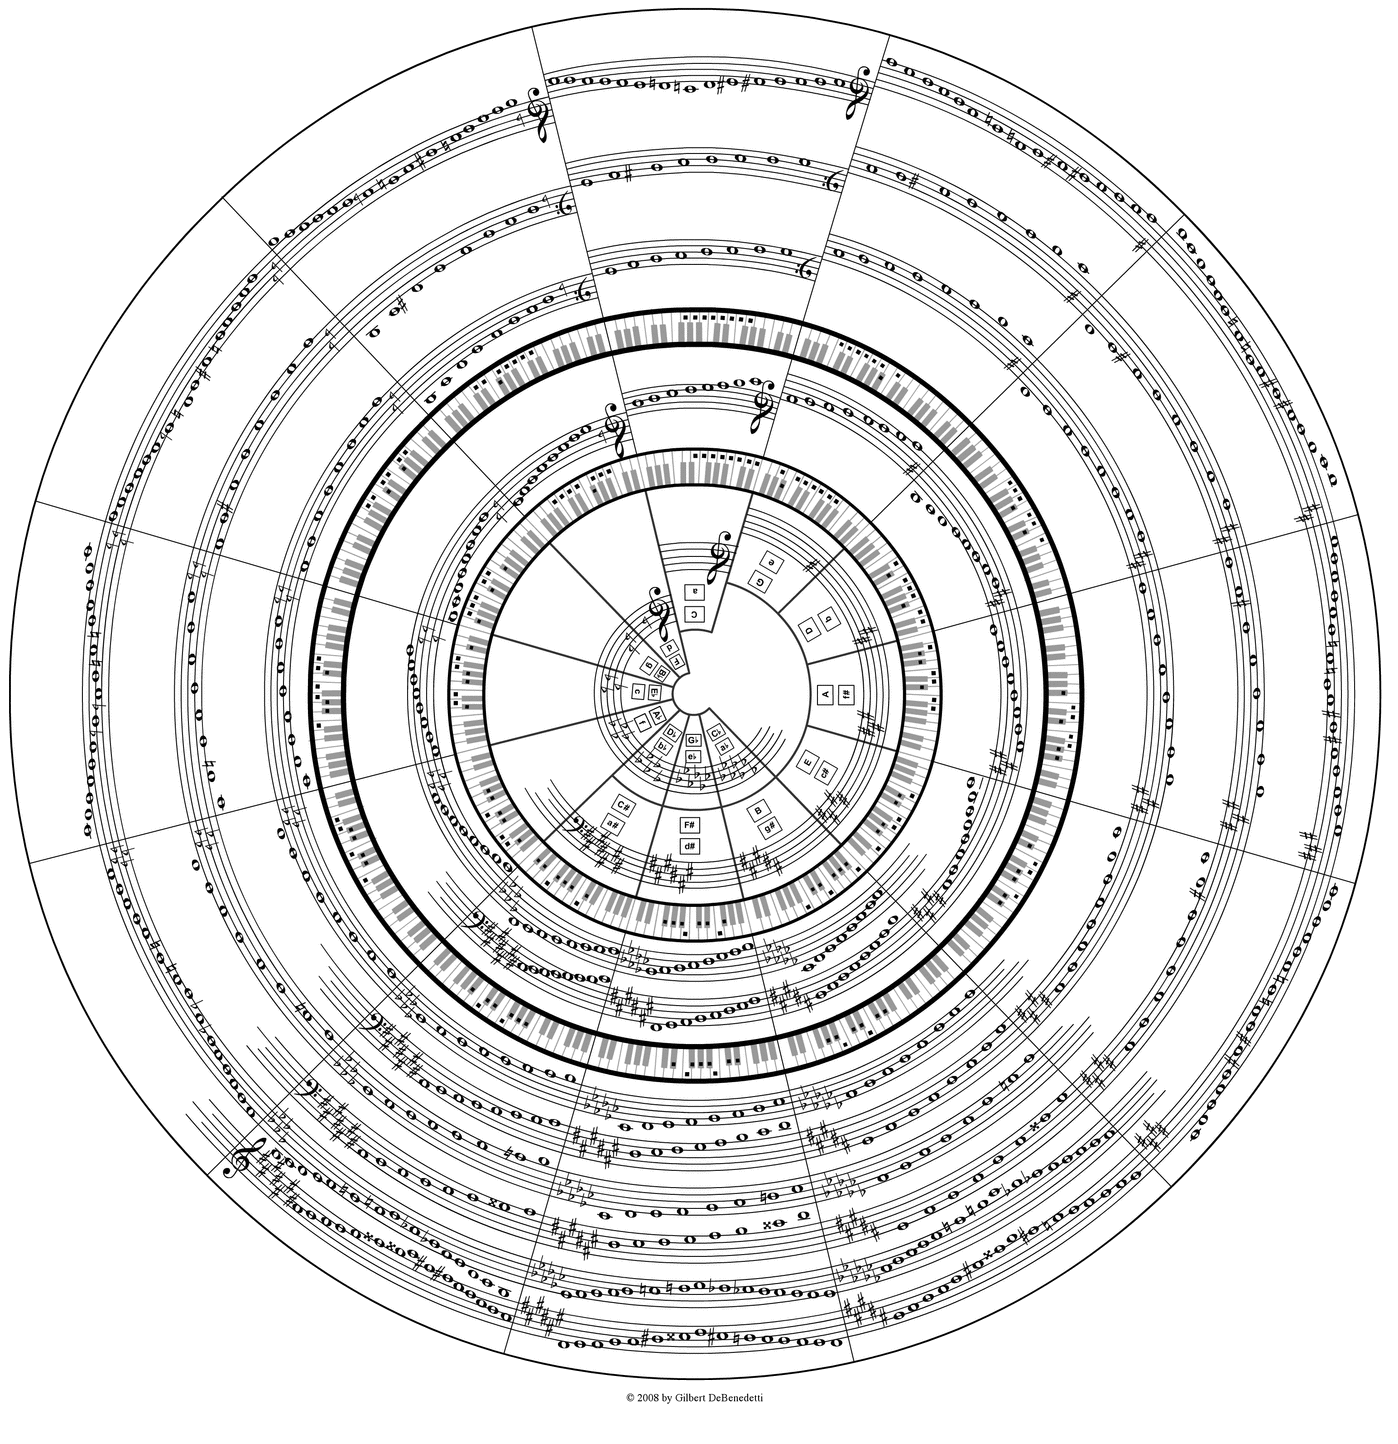
\includegraphics[width=.6\textwidth]{img/cover_img.png}~\\[2cm]
            \vfill

            % Author
            \begin{minipage}{\textwidth}
            \begin{center}\Large
                Rand Asswad\\
                Department of Applied Mathematics
            \end{center}
            \end{minipage} \\[2cm]

            % Author and supervisor
            \begin{minipage}{0.45\textwidth}
            \begin{flushleft} \large
                \emph{INSA tutor:}\\
                Natalie FORTIER
            \end{flushleft}
            \end{minipage}
            \begin{minipage}{0.45\textwidth}
            \begin{flushright} \large
                \emph{Internship supervisors:}\\
                Dario PRANDI\\
                Ugo BOSCAIN
            \end{flushright}
            \end{minipage}

            \vfill
            % Bottom of the page
            {\large 04/01/2021 - 30/06/2021}
        \end{center}
    \end{sffamily}
\end{titlepage}
\makeatother

{
\setcounter{tocdepth}{3}
\tableofcontents
}
\def\R{\mathbb{R}}
\def\C{\mathbb{C}}
\def\N{\mathbb{N}}
\def\Z{\mathbb{Z}}

\def\Cl{\mathcal{C}}
\def\U{\mathcal{U}}
\def\F{\mathcal{F}}
\def\H{\mathbb{H}}

\def\w{\omega}
\let\aphi\phi
\def\phi{\varphi}
\def\epsilon{\varepsilon}
\def\eps{\varepsilon}

\def\numin{\nu_{\min}}
\def\numax{\nu_{\max}}

\def\ddt{\frac{\mathrm{d}}{\mathrm{d}t}}
\def\dx{\mathrm{d}x}
\def\dt{\mathrm{d}t}
\def\ds{\mathrm{d}s}
\def\dtau{\mathrm{d}\tau}
\def\dw{\mathrm{d}\w}
\def\dnu{\mathrm{d}\nu}
\def\dtheta{\mathrm{d}\theta}
\def\dtfrac{\frac{\partial}{\partial t}}

\def\pp#1{\left(#1\right)}
\def\sset#1{\left\{#1\right\}}
\def\vset#1#2{\sset{#1\left\lvert#2\right.}}

\def\abs #1{\left\lvert#1\right\rvert}
\def\norm#1{\left\lVert#1\right\rVert}
\def\dotp#1{\left\langle#1\right\rangle}
\def\round#1{\left\lfloor#1\right\rceil}

\def\bbar#1{\overline{#1}}

\def\pmat#1{\begin{pmatrix}#1\end{pmatrix}}
\def\hmat#1#2{\pmat{#1 & #2\\0 & 1}}

\def\Aut{\mathrm{Aut}}

\def\qtext#1{\quad\text{#1}\quad}

\def\argmin{\mathop{\mathrm{argmin}}}
\def\argmax{\mathop{\mathrm{argmax}}}
\def\supp{\mathop{\mathrm{supp}}}

\def\transp#1{{#1}^{\top}}

\def\stft #1{\mathrm{STFT}\sset{#1}}
\def\STFT{\mathrm{STFT}}
\def\Proj{\mathrm{Proj}}

\def\Cd{\mathrm{Cauchy}}
\def\Nd{\mathcal{N}}
\def\med{\mathrm{median}}

\pagebreak

\hypertarget{acknowledgements}{%
\section*{Acknowledgements}\label{acknowledgements}}
\addcontentsline{toc}{section}{Acknowledgements}

First I would like to thank my supervisors, Dario Prandi and Ugo Boscain
for the great opportunity and their invaluable advice and guidance throughout the internship,
as well as their support along with Giuseppina Turco in my project of persuing a PhD.
I would also like to thank Ludovic Sacchelli along with them for the opportunity
to coauther a paper in the GSI 2021 conference.

I am also extremely grateful to Natalie Fortier for her support during my studies
in the GM department, especially during the last two years.
My thanks extend to the GM professors who have helped me discover my passion
and opened my mind to new horizons.
I would also like to thank the professors of the ITA Master's program
at University of Rouen Normandie, especially Jean-Philippe Dubernard.

Most importantly, I thank my family, without their tremendous support
it would be impossible for me to complete my studies.
My parents for prioritizing our education, Raja and Madeleine
for their unwaivoring support throughout my education,
Jad and Mery for their care and support despite the distance.

Finally, I want to thank my second Rouen family, Ibrahim
my best friend and colleague for his continuous encouragement,
along with Louise, Hajar, and Diane, for the stimulating discussions,
and their help and encouragement.
Last but not least, Sally who was there for me and lifted me up
during the difficult times.

\pagebreak

\hypertarget{introduction}{%
\section{Introduction}\label{introduction}}

\hypertarget{laboratory-and-supervision}{%
\subsection{Laboratory and supervision}\label{laboratory-and-supervision}}

The Laboratory of Signals and Systems (L2S) is a French
research laboratory created in 1974, operated by the CNRS,
CentraleSupélec and the University of Paris-Saclay.

Research at L2S is conducted in fundamental and applied mathematics,
divided into three main fields:
Systems and Control, Signal processing and Statistics,
and Networks and Telecommunications.

My supervisor Dario Prandi, is a member of the COMEDY team
which focuses on analysis of structural properties
and control of classes of dynamical systems.
The main focus is on fundamental results, but with a strong
link to applications {[}\protect\hyperlink{ref-l2s}{30}{]}.

Dario Prandi has been working on a bio-inspired model for sound
reconstruction, along with Ugo Boscain, Ludovic Sacchelli,
and Giuseppina Turco.
Ugo Boscain (CNRS, Inria, Laboratoire Jacques-Louis Lions,
Sorbonne Université) has supervised me closely along with Dario Prandi.

As the intership took place during the COVID-19 pandemic outbreak,
I worked from home.
An open channel on Microsoft Teams allowed us to communicate
whenever it was needed. Moreover, a visio-conference call
was scheduled to discuss the established work and the following tasks.
In addition, whenever we had the chance, an in-person meeting was organized
allowing a prolonged discussion of the on-going work.

\hypertarget{internship-mission}{%
\subsection{Internship mission}\label{internship-mission}}

The goal of the internship is to carry out the work that had been started
on the sound reconstruction model, which needed at that point
numerical and theoretical validation.

Preliminary tests were carried out on synthetic sounds, giving promising results.
Nevertheless, tests on real speech signals were needed as the model
was conceived for that purpose.
The course of the internship would be decided depending on the numerical validation.
As it turned out, a new mathematical approach was needed in order
to improve the model.

\pagebreak

\hypertarget{image-reconstruction-model}{%
\section{Image reconstruction model}\label{image-reconstruction-model}}

The geometric model for sound reconstruction was inspired by
a sub-Riemannian model of the visual cortex V1 for image reconstruction.
Therefore, a preliminary study of the image reconstruction was needed
in order to understand the sound model and the challenges that are
faced in adapting the initial model for sound reconstruction.

\hypertarget{neoro-geometric-model-of-v1}{%
\subsection{Neoro-geometric model of V1}\label{neoro-geometric-model-of-v1}}

My supervisors and their colleagues have presented a cortical-inspired
image reconstruction algorithm {[}\protect\hyperlink{ref-bertalmio2018}{3},\protect\hyperlink{ref-boscain2017}{4}{]} based
on the Citti-Petitot-Sarti (CPS) model of the human primary visual cortex V1 {[}\protect\hyperlink{ref-citti2006}{8},\protect\hyperlink{ref-petitot1999}{21}{]}.

The CPS model is based on the work of Hubel and Wiesel {[}\protect\hyperlink{ref-hubel1959}{16}{]} who observed that there are
groups of neurons sensitive to positions and directions.
This has inspired Hoffman {[}\protect\hyperlink{ref-hoffman1989}{15}{]} to model V1 as a contact space
(a three-dimensional manifold endowed with a smooth map).
Since an image can be seen as a function \(f:\mathbb{R}^2\rightarrow\mathbb{R}_+\) representing
the grey level at given coordinates, the visual cortex adds
the angle \(\theta\in P^1\) of the tangent line to the curve,
where \(P^1=\mathbb{R}/\pi\mathbb{Z}\) is the projective line of non-directed angles.
The model therefore lifts the image into \(\mathbb{R}^2\times P^1\).

\hypertarget{wilson-cowan-model-in-v1}{%
\subsection{Wilson-Cowan model in V1}\label{wilson-cowan-model-in-v1}}

The Wilson-Cowan (WC) model {[}\protect\hyperlink{ref-wilson1972}{26}{]} describes the evolution of neural activations,
more precisely, it describes the evolution of excitatory and inhibitory activity in
a synaptically coupled neuronal network.

The interaction between the hypercolumns in V1 can be described through
the WC equations {[}\protect\hyperlink{ref-bressloff2002}{6}{]}.
An integro-differential equation describing the state \(a(x,\theta,t)\) of a population
of neurons with V1 coordinates \(x\in\mathbb{R}^2\) and orientation \(\theta\in P^1\) at time \(t>0\) {[}\protect\hyperlink{ref-bertalmio2018}{3}{]}.

\begin{equation}
\frac{\partial}{\partial t}a(x,\theta,t) = -\alpha a(x,\theta,t) + \nu
\int_{\mathbb{R}^2\times P^1} \omega(x,\theta\| x',\theta') \sigma(a(x',\theta',t)) \mathrm{d}x'\mathrm{d}\theta'
+ h(x,\theta,t)
\end{equation}

\begin{figure}[H]
    \centering
    \begin{minipage}{0.3\linewidth}
        \centering
        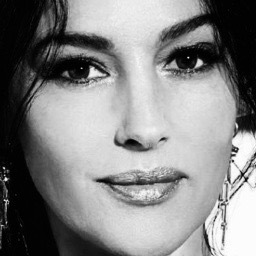
\includegraphics[width=\textwidth]{img/img_original.jpg}\\original
    \end{minipage}\hfill%
    \begin{minipage}{0.3\linewidth}
        \centering
        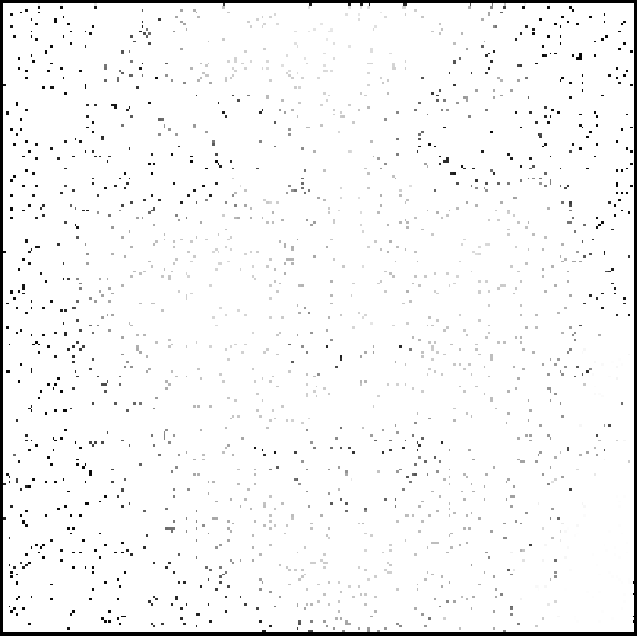
\includegraphics[width=\textwidth]{img/img_corrupted.png}\\corrupted
    \end{minipage}\hfill%
    \begin{minipage}{0.3\linewidth}
        \centering
        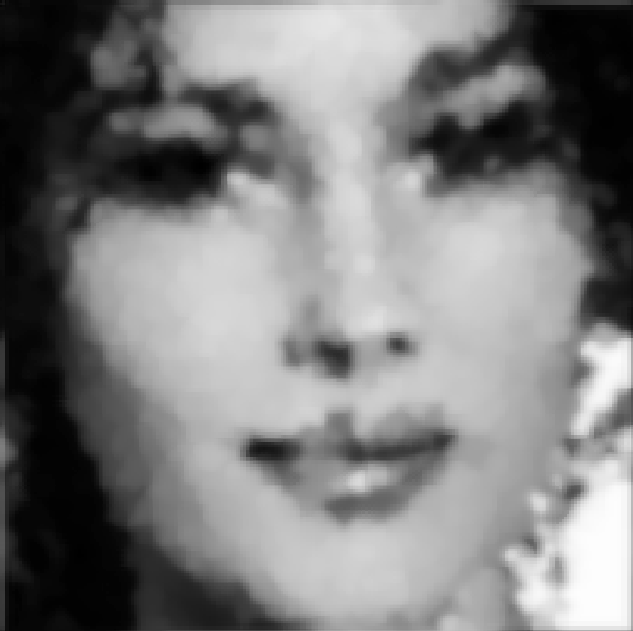
\includegraphics[width=\textwidth]{img/img_reconstructed.png}\\reconstructed
    \end{minipage}
    \caption{Reconstruction of a 97\% corrupted image}
    \label{fig:img-reconstruct}
\end{figure}

\pagebreak

\hypertarget{sound-reconstruction-model}{%
\section{Sound reconstruction model}\label{sound-reconstruction-model}}

\hypertarget{from-v1-to-a1}{%
\subsection{From V1 to A1}\label{from-v1-to-a1}}

The motivation behind the application of the model in sound reconstruction
is the idea that a sound can be seen as an image in the time-frequency domain.
The primary auditory cortex A1 receives the sensory input directly from the cochlea {[}\protect\hyperlink{ref-dallos1996}{10}{]},
which is a spiral-shaped fluid-filled cavity that composes the inner ear.

The mechanical vibrations along the basilar membrane are transduced into electrical activity
along a dense, topographically ordered, array of auditory-nerve fibers
which convey these electrical potentials to the central auditory system.

Since these auditory-nerve fibers (sensors or inner hair cells) are topographically ordered
along the cochlea spiral, different regions of the cochlea are sensitive to different frequencies.
Hair cells close to the base are more sensitive to low-frequency sounds and those near the apex
are more sensitive to high-frequency sounds {[}\protect\hyperlink{ref-yang1992}{27}{]}.

\begin{figure}
\centering
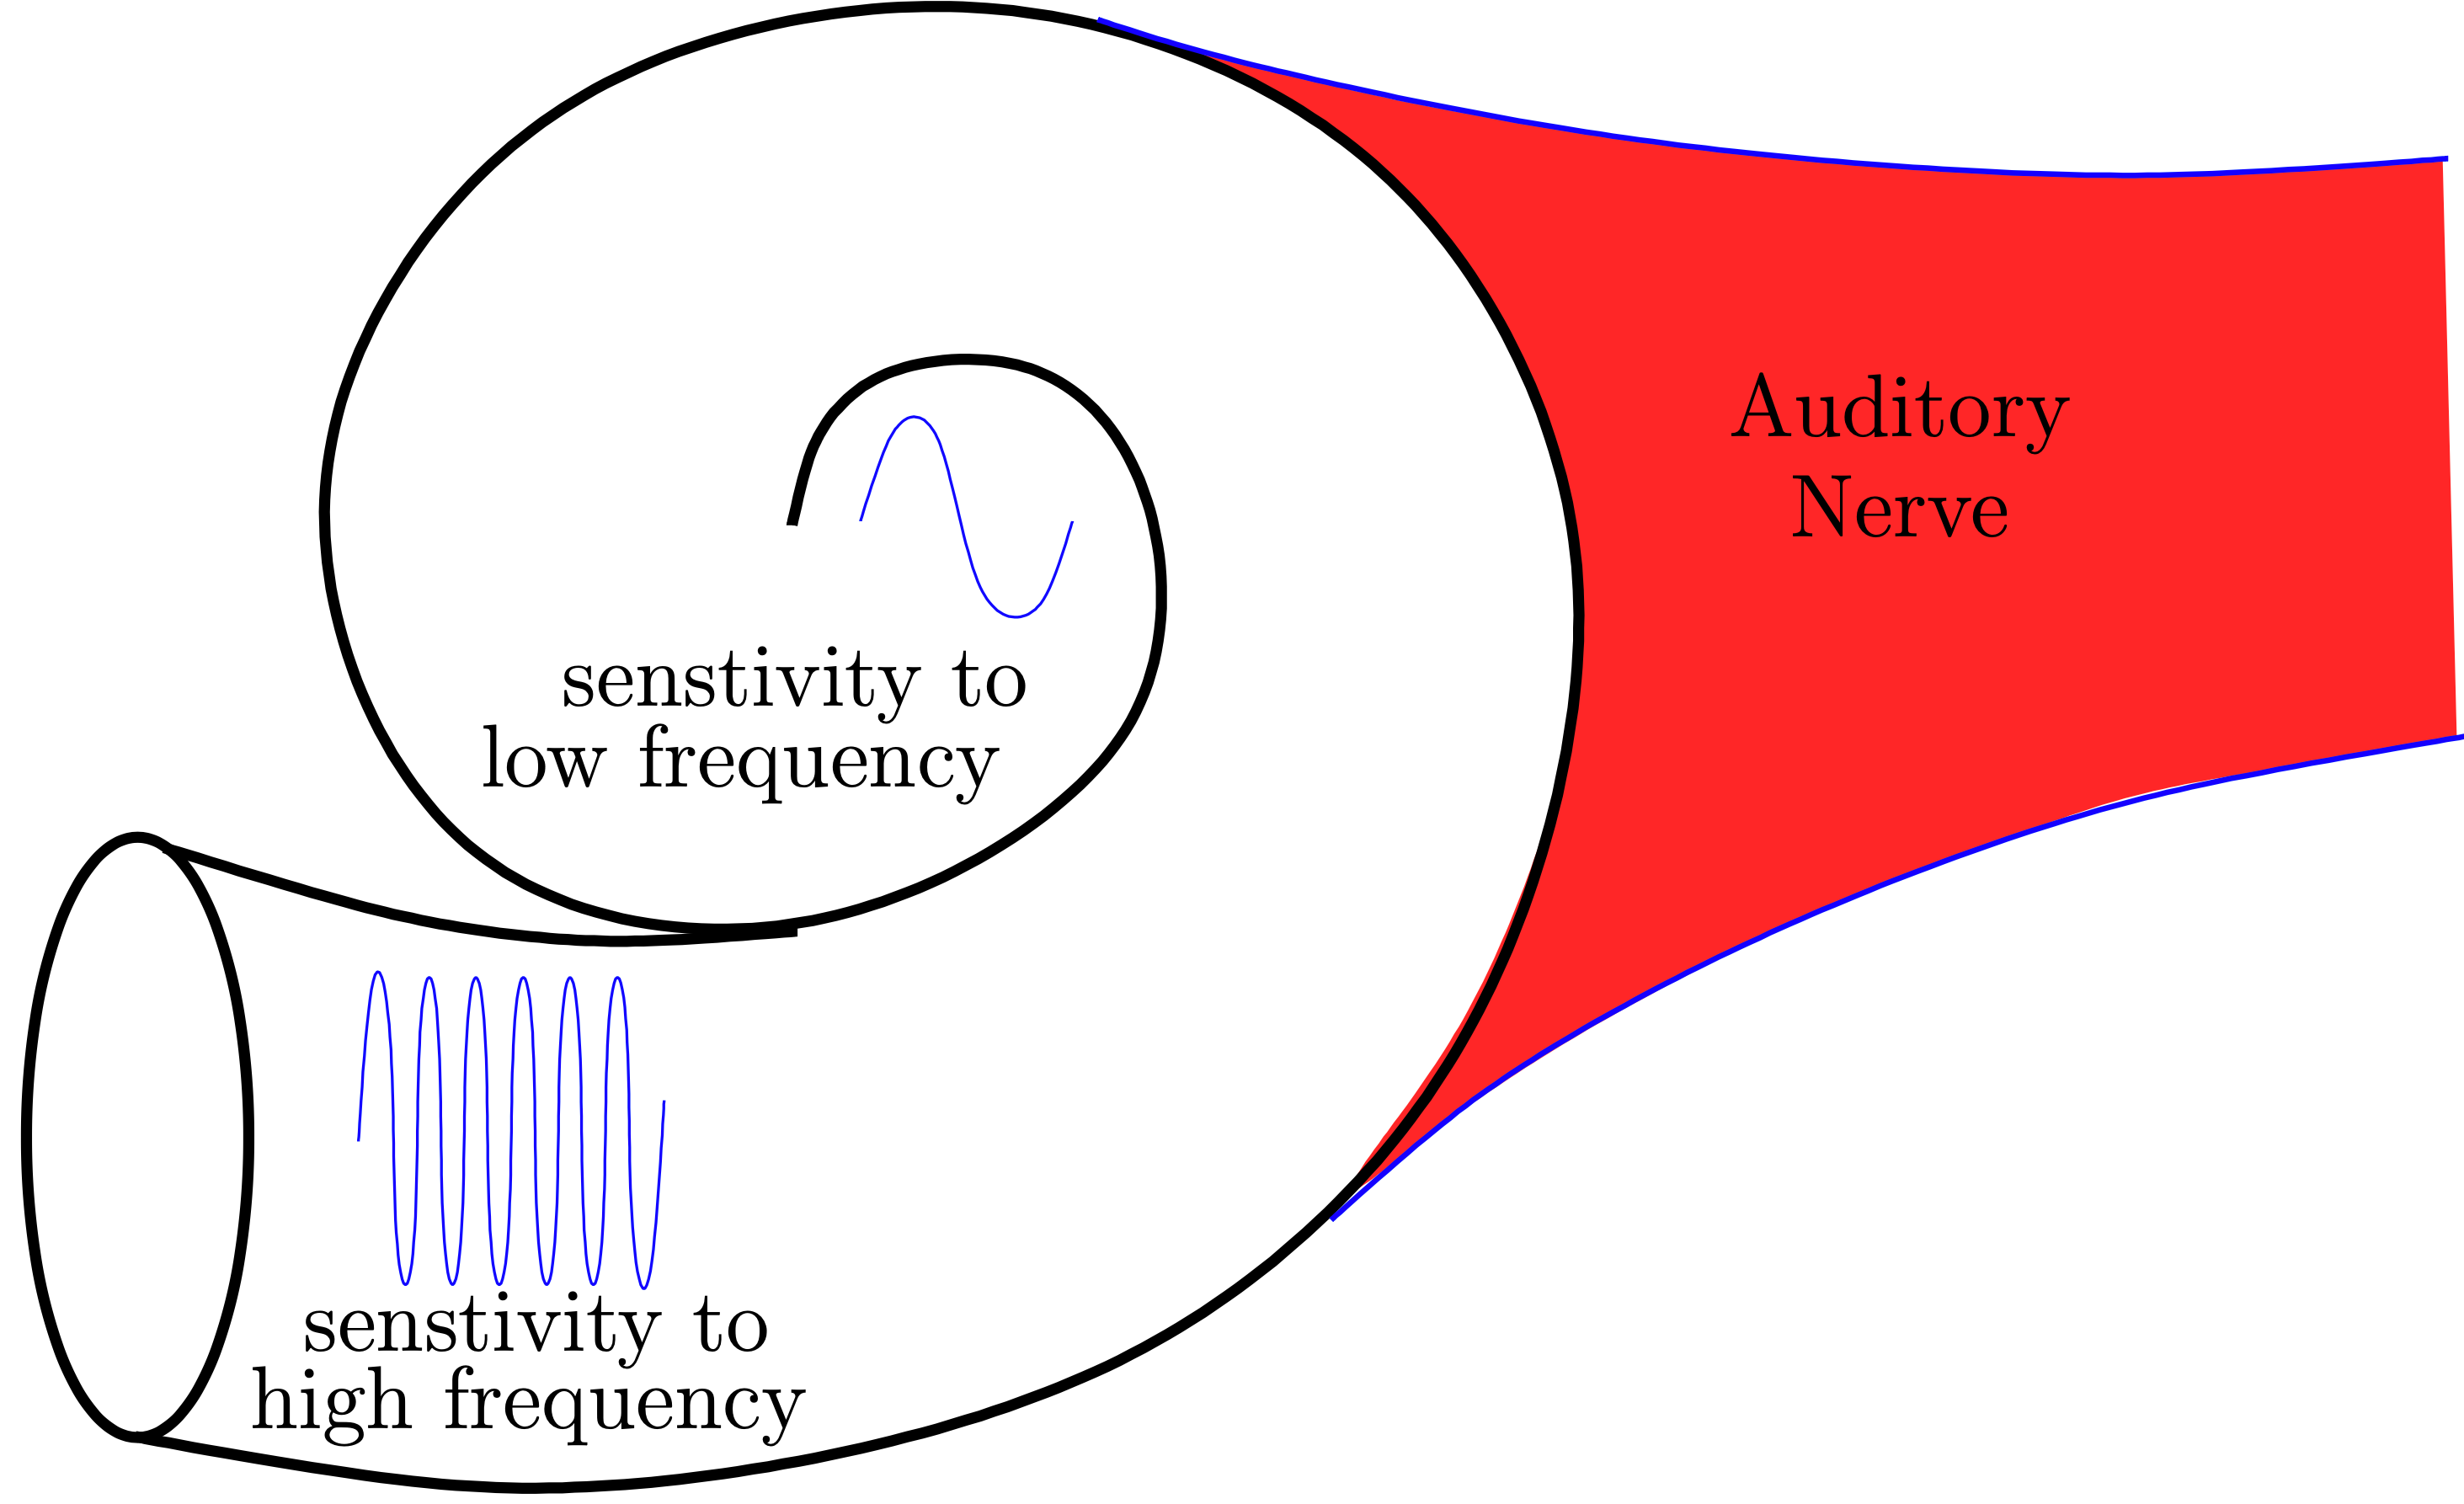
\includegraphics[width=0.5\textwidth,height=\textheight]{img/cochlea.png}
\caption{Perceived pitch of a sound depends on the location in the cochlea that the sound wave stimulated {[}\protect\hyperlink{ref-boscain2021}{5}{]}.}
\end{figure}

This spatial segregation of frequency sensitivity in the cochlea
means that the primary auditory cortex receives a time-frequency representation of the sound.
In this model, we consider the Short-Time Fourier Transform (STFT)
as the time-frequency representation \(S(\tau,\omega)\) of a sound signal \(s\in L^2(\mathbb{R})\)

While the spectrogram of a sound signal \(\left\lvert S\right\rvert(\tau,\omega)\) is an image,
the image reconstruction algorithm cannot be applied to a corrupted sound
since the rotated spectrogram would correspond to completely different input sound
therefore the invariance by rototranslation is lost.
Moreover, the image reconstruction would evolve the WC equation on the entire
image simultaneously. However, the sound image (spectrogram) does not reach
the auditory cortex simultaneously but sequentially.
Hence, the reconstruction can be performed only in a sliding window {[}\protect\hyperlink{ref-boscain2021}{5}{]}.

\hypertarget{sound-reconstruction-pipeline}{%
\subsection{Sound reconstruction pipeline}\label{sound-reconstruction-pipeline}}

As discussed in the previous section, the sound reconstruction model
is inspired by the V1 model.
First, a 2-dimensional image of the sound signal is obtained via a short-time Fourier transform,
which is analogous to the spectrogram the cochlea transmits to the auditory cortex.
The time derivative of the frequency \(\nu=\mathrm{d}\omega/\mathrm{d}\tau\), corresponding to the chirpiness of the sound,
allows adding a new dimension to the sound image.
Afterwards, the sound image is lifted into an \emph{augmented space} that is \(\mathbb{R}^3\)
with the Heisenberg group structure.
Henceforth, the sound is processed in its 3D representation,
that is the obtained lift \(L(\tau,\omega,\nu)\).

Similarly to the V1 model, the sound is reconstructed by solving
the Wilson-Cowan integro-differential equation.

Finally, the solution to the Wilson-Cowan equations is projected into
the time-frequency representation which gives a sound signal through
an inverse short-time Fourier transform {[}\protect\hyperlink{ref-boscain2021}{5}{]}.

\begin{figure}
\centering
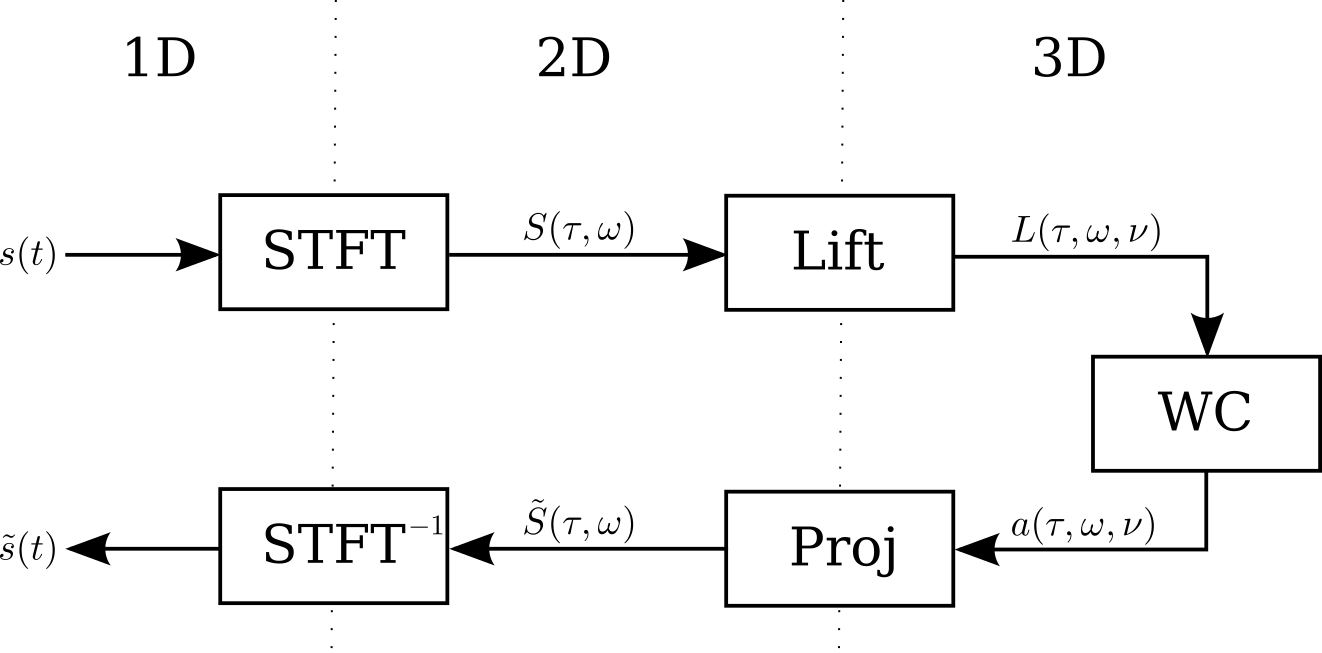
\includegraphics[width=0.7\textwidth,height=\textheight]{img/pipeline.png}
\caption{Sound reconstruction pipeline}
\end{figure}

\hypertarget{time-frequency-representation}{%
\subsection{Time-Frequency representation}\label{time-frequency-representation}}

The Fourier transform transforms a time signal \(s\in L^2(\mathbb{R})\)
into a complex function of frequency \(\hat s\in L^2(\mathbb{R})\).
Since the time signal \(s\) can be obtained from \(\hat s\)
using the Inverse Fourier Transform, they both contain
the exact same information.
Conceptually, \(s\) and \(\hat s\) can be considered two equivalent
representations of the same object \(s\), but each one
makes visible different features of \(s\).

A time-frequency representation would combine the features
of both \(s\) and \(\hat s\) into a single function.
Such representation provides an \emph{instantaneous frequency spectrum}
of the signal at any given time {[}\protect\hyperlink{ref-grochenig2001}{13}{]}.

\hypertarget{the-short-time-fourier-transform}{%
\subsubsection{The Short-Time Fourier Transform}\label{the-short-time-fourier-transform}}

The Short-Time Fourier Transform (STFT) is a very common
Time-Frequency representation of a signal.
The principle of the STFT is quite straightforward.
In order to obtain a Time-Frequency representation of a signal \(s\),
a Fourier transform is taken over a restricted interval
of the original signal \emph{sequentially}.
Since a sharp cut-off introduces discontinuities and aliasing issues,
a smooth cut-off is prefered {[}\protect\hyperlink{ref-grochenig2001}{13}{]}.
This is established by multiplying a segment of the signal by a weight function,
that is smooth, compactly supported, and centered around \(0\),
referred to as \emph{window}.
Essentially, the STFT \(S(\tau,\omega)\) is the Fourier transform of \(s(t)w(t-\tau)\)
(the signal taken over a sliding window along the time axis.)

\begin{equation}
S(\tau,\omega) = \int_\mathbb{R}s(t)w(t-\tau)e^{-2\pi i\omega t} \mathrm{d}t
\end{equation}

\begin{figure}
\centering
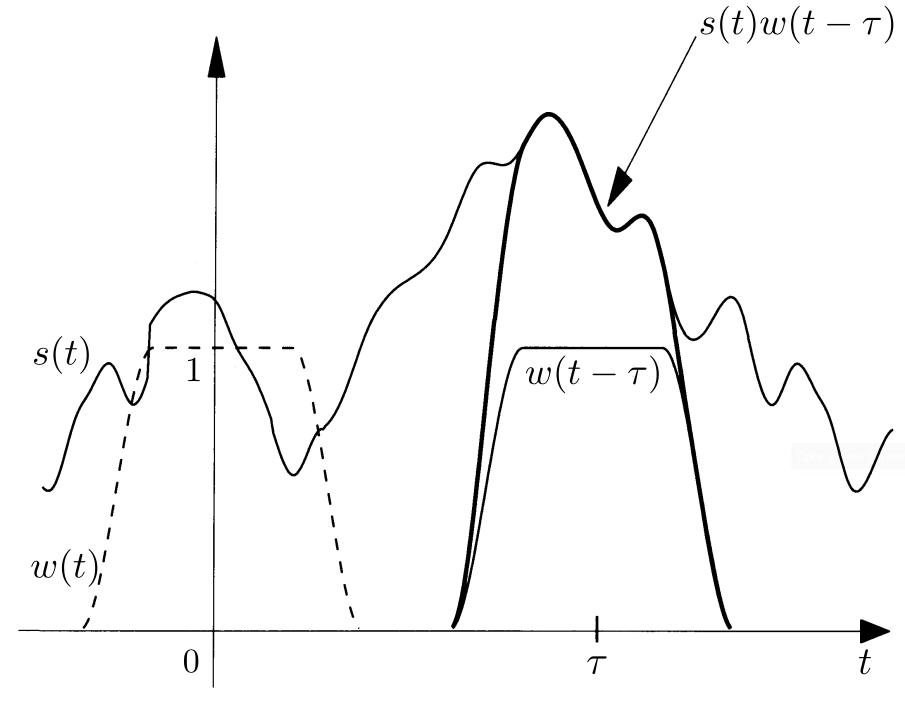
\includegraphics[width=0.4\textwidth,height=\textheight]{img/stft_grochenig.png}
\caption{Signal windowing for the STFT {[}\protect\hyperlink{ref-grochenig2001}{13}{]}}
\end{figure}

\hypertarget{time-and-frequency-shifts-operators}{%
\subsubsection{Time and frequency shifts operators}\label{time-and-frequency-shifts-operators}}

In our study, we consider realizable signals \(s\in L^2(\mathbb{R})\).
Fundamental operators in time-frequency analysis are
time and phase shifts acting on realizable signals \(s\in L^2(\mathbb{R})\).

\begin{itemize}
\tightlist
\item
  \textbf{Time shift operator:} \(T_\tau s(t)=s(t-\tau)\)
\item
  \textbf{Phase shift operator:} \(M_\omega s(t)=e^{2\pi i \omega t} s(t)\)
\end{itemize}

We notice that the STFT can be formulated using these unitary operators

\begin{align}
S(\tau,\omega) &= \int_\mathbb{R}s(t)w(t-\tau)e^{-2\pi i\omega t} \mathrm{d}t\\
    &= \int_\mathbb{R}s(t) \overline{M_\omega T_\tau w(t)} \mathrm{d}t\\
    &= \left\langle s, M_\omega T_\tau w\right\rangle_{L^2(\mathbb{R})}
\end{align}

We can redefine the STFT as an operator \(V_w\) on \(s\in L^2(\mathbb{R})\)
defined in function of \(T_\tau\) and \(M_\omega\) {[}\protect\hyperlink{ref-boscain2021}{5},\protect\hyperlink{ref-grochenig2001}{13}{]}.

\begin{equation}\label{eq:stft_operator}
V_w s(\tau,\omega) = \left\langle s, M_\omega T_\tau w\right\rangle_{L^2(\mathbb{R})}
\end{equation}

\hypertarget{discrete-stft}{%
\subsubsection{Discrete STFT}\label{discrete-stft}}

Similarly to the continuous STFT, the discrete STFT is the
Discrete Fourier Transform (DFT) of the signal over a sliding window.
Nevertheless, the window cannot slide continuously along the time axis,
instead the signal is windowed at different frames with an overlap.
The window therefore hops along the time axis.

Let \(N\) be the window size (DFT size), we define the overlap \(R\)
as the number of overlapping frames between two consecutive windows.
The hop size is therefore defined as \(H=N-R\).
We also define the overlap ratio as the ratio of the overlap
with respect to the window size \(r=R/N\) where \(r\in[0,1[\).

The discrete STFT of a signal \(s\in L^2([0,T])\) is therefore
\begin{equation}
S[m,\omega] = \sum_{t=0}^{T} s[t]w[t-mH]e^{-2\pi i\omega t}
\end{equation}

The choice of parameters has direct influence over the discrete STFT
resolution, as well as its invertibility.

\hypertarget{stft-windowing}{%
\subsubsection{STFT windowing}\label{stft-windowing}}

The choice of the window affects quality of the Fourier transform.
One should choose a window with anti-aliasing and that distributes
spectral leakage.

\begin{figure}[H]
    \centering
    \begin{subfigure}[t]{\textwidth}
        \centering
        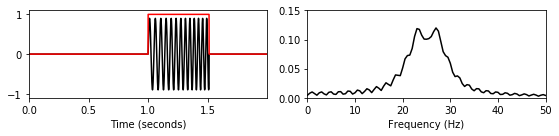
\includegraphics[width=0.6\textwidth]{img/w_rectangle.png}
        \caption{Rectangular window}
    \end{subfigure}
    \begin{subfigure}[t]{\textwidth}
        \centering
        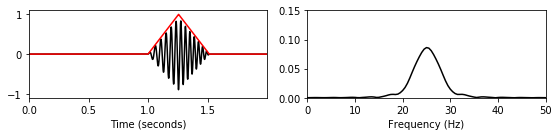
\includegraphics[width=0.6\textwidth]{img/w_triangle.png}
        \caption{Triangular window}
    \end{subfigure}
    \begin{subfigure}[t]{\textwidth}
        \centering
        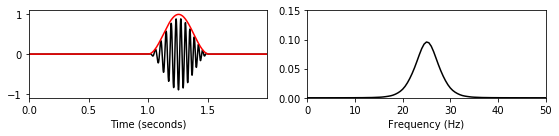
\includegraphics[width=0.6\textwidth]{img/w_hann.png}
        \caption{Hann window}
    \end{subfigure}
    \caption{Different windows (left) and their respective Fourier transform (right)}
\end{figure}

Moreover, as we will see in the next sections, the STFT is invertible.
However, the STFT parameters need to satisfy the two following constraints {[}\protect\hyperlink{ref-griffin1983}{12},\protect\hyperlink{ref-muller2015}{19}{]}:

\begin{itemize}
\tightlist
\item
  \textbf{Nonzero OverLap Add (NOLA):} \(\sum\limits_{m\in\mathbb{Z}} w^2[t-mH] \neq 0\)
\item
  \textbf{Constant OverLap Add (COLA):} \(\sum\limits_{m\in\mathbb{Z}} w[t-mH] = 1\)
\end{itemize}

The NOLA condition is met for any window given an overlap ratio \(r\in[0,1[\).
It is worth noting that this condition can be found without the square
depending on the inverse STFT algorithm.

The COLA constraint defines the partition of unity over the discrete time axis,
imposing a stronger condition.

\begin{figure}[H]
    \centering
    \begin{subfigure}[t]{\textwidth}
        \centering
        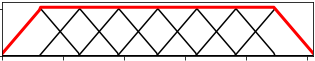
\includegraphics[width=0.45\textwidth]{img/woa_triangular_1_2.png}
        \caption{Triangular window, overlap ratio $r=\frac{1}{2}$}
    \end{subfigure}
    \begin{subfigure}[t]{\textwidth}
        \centering
        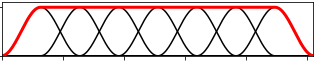
\includegraphics[width=0.45\textwidth]{img/woa_hann_1_2.png}
        \caption{Hann window, overlap ratio $r=\frac{1}{2}$}
    \end{subfigure}
    \begin{subfigure}[t]{\textwidth}
        \centering
        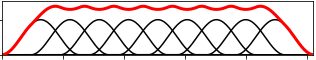
\includegraphics[width=0.45\textwidth]{img/woa_hann_3_8.png}
        \caption{Hann window, overlap ratio $r=\frac{3}{8}$}
    \end{subfigure}
    \caption{The COLA condition with different windows and overlap ratios}
\end{figure}

In typical applications, the window functions used are non-negative,
smooth, bell-shaped curves {[}\protect\hyperlink{ref-roads2002}{24}{]}.
A comprehensive list of windows and their properties may be found in {[}\protect\hyperlink{ref-heinzel2002}{14}{]}.
In our model we use the Hann window, which satisfies the COLA condition
for any overlap ratio of \(r=\frac{n}{n+1},n\in\mathbb{N}^*\).

The Hann window of length \(L\) is defined as
\begin{equation}
w(x)=\begin{cases}
\frac{1+\cos\left(\frac{2\pi x}{L}\right)}{2} & \text{if}~\left\lvert x\right\rvert\leq\frac{L}{2}\\
0 & \text{if}~\left\lvert x\right\rvert>\frac{L}{2}
\end{cases}
\end{equation}

\hypertarget{uncertainty-principle-and-resolution-issues}{%
\subsubsection{Uncertainty principle and resolution issues}\label{uncertainty-principle-and-resolution-issues}}

As previously stated, both \(s\) and \(\hat s\) contain the exact same information.
However, there is a fundamental limit to the accuracy with which the values
for certain pairs of physical pairs can be observed.
A known example to issue is Heisenberg's uncertainty principle regarding
the position of a particle and its momentum {[}\protect\hyperlink{ref-sen2014}{25}{]}.
Similarly, time and frequency are a pair of complementary variables.

In the context of time-frequency analysis, the Heisenberg-Gabor limit
(or simply the Gabor limit) defines this constraint by the following inequality

\begin{equation}
\sigma_t\cdot\sigma_\omega\geq \frac{1}{4\pi}
\end{equation}
where \(\sigma_t\) and \(\sigma_\omega\) are the standard deviations of the time and frequency respectively.

The Gabor limit means essentially that
``a realizable signal occupies a region of area at least one in the time-frequency plane.''
Which means that we cannot sharply localize a signal in both the time domain and frequency domain.
This makes the concept of an instantaneous frequency impossible {[}\protect\hyperlink{ref-grochenig2001}{13}{]}.

A direct result of the uncertainty principle is the fact that high temporal resolution
and frequency resolution cannot be acheived at the same time.

\begin{figure}
\centering
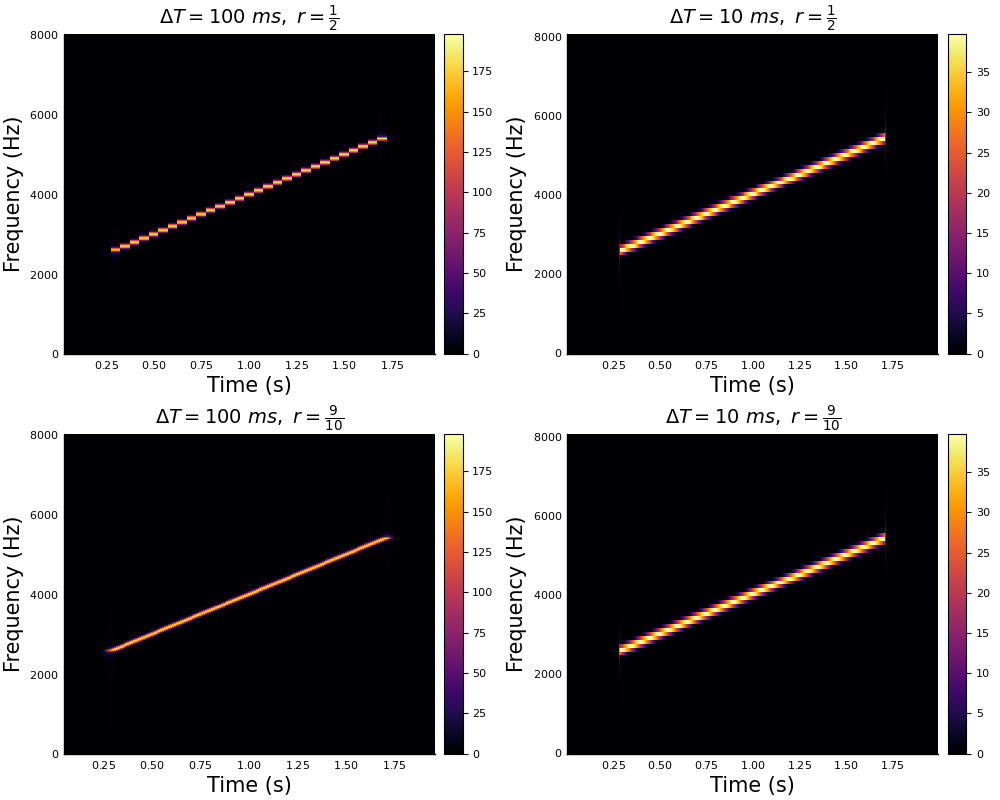
\includegraphics{img/stft_resolution.png}
\caption{STFT resolution with respect to different window sizes \(\Delta T\) and overlap ratios \(r\)}
\end{figure}

In the figure above, we see the influence of the window size and the overlap ratio on the
STFT resolution.

\begin{itemize}
\tightlist
\item
  \textbf{Window size:}
  For larger window sizes, we have higher frequency resolution. However, the time resolution is low as we have fewer time samples for the STFT.
  For smaller windows, we get higher time resolution as we have more time samples for the STFT, while losing frequency resolution due to smaller FT size.
\item
  \textbf{Overlap:}
  In the case of smaller overlaps, the resulting spectrum has time discontinuities. Indeed, the straight line appears to be a piece-wise constant function of time.
  For overlap ratios close to 1, the time resolution is significantly better obtaining the best results (given an adequate window size). However, one should keep in mind that high overlaps can be computationally costly.
\end{itemize}

\hypertarget{inverse-short-time-fourier-transform}{%
\subsubsection{Inverse Short-Time Fourier Transform}\label{inverse-short-time-fourier-transform}}

The operator \(V_w\) is an isometry from \(L^2(\mathbb{R})\) to \(L^2(\mathbb{R}^2)\)
if \(\left\lVert w\right\rVert_2=1\),
allowing for \(s\) to be completely determined by \(V_w s\).
With the help of the orthogonality relations (Parseval's formula) on the STFT we obtain
the inversion formula for the STFT (see Appendix \ref{istft} for a detailed proof).

For \(w,h\in L^2(\mathbb{R})\) smooth windows such that \(\left\langle w,h\right\rangle\neq 0\)
we have for all \(s\in L^2(\mathbb{R})\),

\begin{align}
s(t) &=\frac{1}{\left\langle w,h\right\rangle} \iint_{\mathbb{R}^2}V_w s(\tau,\omega)M_\omega T_\tau h(t) \mathrm{d}\omega\mathrm{d}\tau\\
     &= \frac{1}{\left\langle w,h\right\rangle}
        \iint_{\mathbb{R}^2} S(\tau,\omega) h(t-\tau) e^{2\pi i\omega t} \mathrm{d}\omega\mathrm{d}\tau
\end{align}

\hypertarget{griffin-lim-algorithm}{%
\subsubsection{Griffin-Lim Algorithm}\label{griffin-lim-algorithm}}

The practical use of the inverse STFT is to obtain the signal
from a spectrum that has undergone some changes.
Daniel W. Griffin and Jae S. Lim {[}\protect\hyperlink{ref-griffin1983}{12}{]} proposed
an efficient algorithm for signal estimation from the modified STFT.
The GLA algorithm minimizes the mean squared error between the STFT magnitude
of the estimated signal and the modified STFT magnitude.

This method is efficient and easy to implement, and is widely
used in signal processing libraries.

Let \(x\in L^2(\mathbb{R})\) be a realizable signal and \(X=V_w x\in L^2(\mathbb{R}^2)\)
be its STFT. Let \(Y\in L^2(\mathbb{R}^2)\) denote the modified STFT.
It's worth noting that \(Y\), in general, is not necessarily an STFT
in the sense that there might not be a signal \(y\in L^2(\mathbb{R})\)
whose STFT is \(Y=V_w y\) {[}\protect\hyperlink{ref-griffin1983}{12}{]}.

Let \(y_\tau \in L^2(\mathbb{R}^2)\) the inverse Fourier transform of \(Y\)
with respect to the frequency \(\omega\) (its second variable)
at a fixed time \(\tau\in\mathbb{R}\).

\begin{equation}
y_\tau(t) = \int_{\mathbb{R}} Y(\tau,\omega) e^{2\pi i\omega t} \mathrm{d}\omega
\end{equation}

The algorithm finds iteratively the signal \(x\) that minimizes
the distance between \(X\) and \(Y\). The distance measure between
the two spectrums is defined as the norm of the difference
over the \(L^2(\mathbb{R}^2)\) space

\begin{equation}
d(X,Y) = \left\lVert X-Y\right\rVert_2^2
    = \iint_{\mathbb{R}^2} \left\lvert X(\tau,\omega) - Y(\tau,\omega)\right\rvert^2 \mathrm{d}\omega\mathrm{d}\tau
\end{equation}

Which is expressed for discrete STFT as
\begin{equation}
d(X,Y) = \sum_\tau \sum_\omega\left\lvert X[\tau,\omega] - Y[\tau,\omega]\right\rvert^2
\end{equation}

The signal \(x[t]\) is therefore reconstructed iteratively along the formula
\begin{equation}
x[t] = \frac{\sum\limits_\tau y_\tau[t]w[t-\tau]}{\sum\limits_\tau w^2[t-\tau]}
\end{equation}

\hypertarget{the-lift-to-the-augmented-space}{%
\subsection{The lift to the augmented space}\label{the-lift-to-the-augmented-space}}

In order to study the Wilson-Cowan model for neural activations,
we need to have a 3D representation of the sound.
In this section we will explain how the STFT of the sound signal
is lifted into the \textbf{contact space} and explore the properties of this space.

\hypertarget{the-sound-chirpiness}{%
\subsubsection{The sound chirpiness}\label{the-sound-chirpiness}}

The 3D representation of the image in the sub-Riemannian model of V1
was obtained by considering the \emph{sensitivity to directions}
represented by an angle \(\theta\in P^1=\mathbb{R}/\pi\mathbb{Z}\).

We transpose this concept of sensitivity to directions
for sound signals to sensitivity to \emph{instantaneous chirpiness}
that is the time derivative of the frequency \(\nu=\mathrm{d}\omega/\mathrm{d}\tau\).
The time derivative of the frequency is indeed the slope
of the tangent line in the sound spectrogram.
Hence establishing the bridge with the visual model.

\hypertarget{single-time-varying-frequency}{%
\subsubsection{Single time-varying frequency}\label{single-time-varying-frequency}}

As we study the sound through its instantaneous frequency and chirpiness,
we consider both the frequency and the chirpiness functions of time.
To properly define the lift, we consider the following single
time-varying frequency sound signal

\begin{equation}
s(t) = A\cdot\sin(\omega(t)t),\quad A\in\mathbb{R}
\end{equation}

The STFT of this signal can be therefore expressed as

\begin{equation}
S(\tau,\omega) = \frac{A}{2i}\left(\delta_0(\omega-\omega(\tau)) - \delta_0(\omega+\omega(\tau))\right)
\end{equation}

supposing the FT is normalized, where \(\delta_0\) is the Dirac delta
distribution centered at 0.
Which means that \(S\) is concentrated on the curves \(\tau\mapsto(\tau,\omega(\tau))\)
and \(\tau\mapsto(\tau,-\omega(\tau))\).

\begin{figure}
\centering
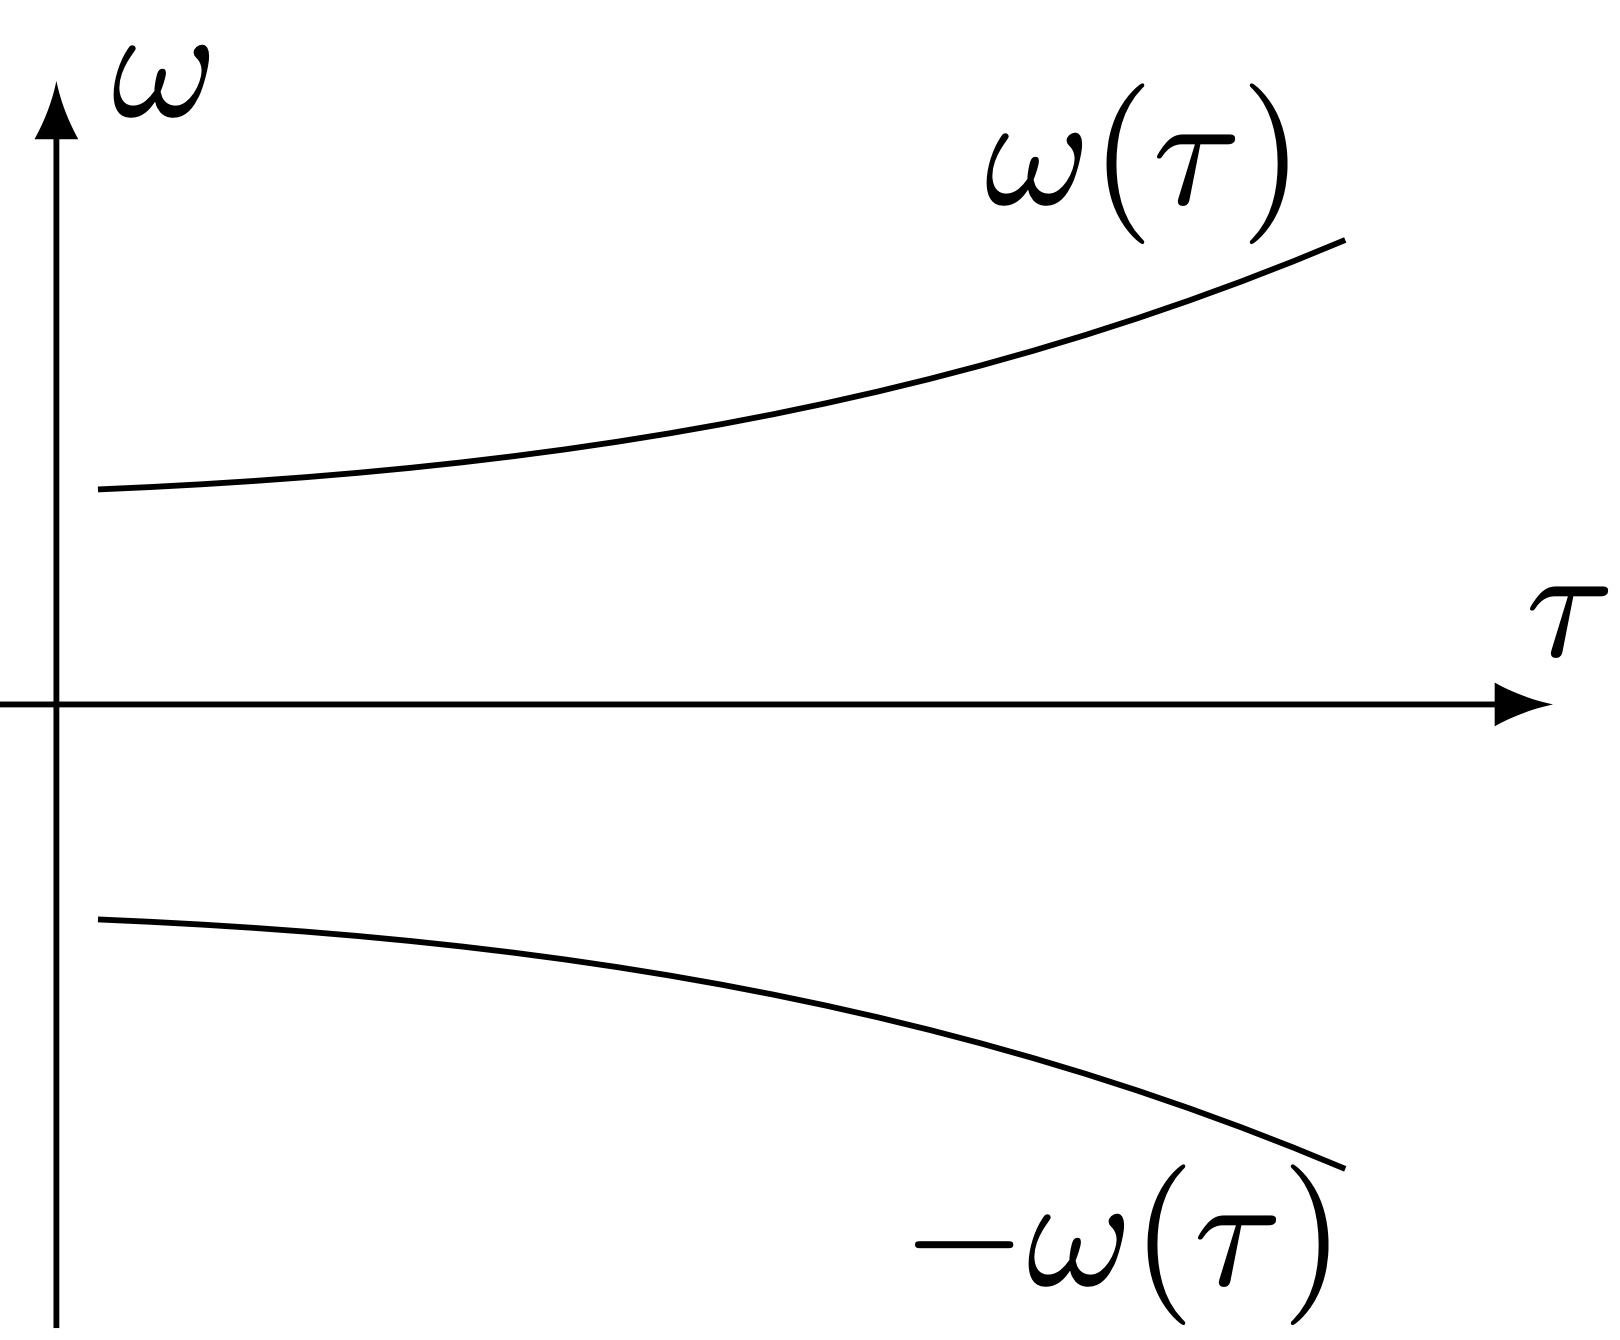
\includegraphics[width=0.25\textwidth,height=\textheight]{img/single_freq.png}
\caption{The STFT the single time-varying frequency sound signal}
\end{figure}

So far, the sound signal is represented in the 2-dimensional space
by the parametric curve \(t\mapsto(t,\omega(t))\).
Nevertheless, we aim to lift our signal into the 3-dimensional \emph{augmented space}
by adding the sensitivity to frequency variations \(\nu(t)=\mathrm{d}\omega(t)/\mathrm{d}t\).
Similarly, the lifted curve is parameterized as \(t\mapsto(t,\omega(t),\nu(t))\) {[}\protect\hyperlink{ref-boscain2021}{5}{]}.

\hypertarget{control-system}{%
\subsubsection{Control system}\label{control-system}}

We define the control to the chirpiness variable \(u(t)=\mathrm{d}\nu/\mathrm{d}t\),
we can therefore say that the curve \(t\mapsto(\tau(t),\omega(t),\nu(t))\)
in the contact space is a lift of a planar curve if there exists
a control \(u(t)\) such that

\begin{equation}
\frac{\mathrm{d}}{\mathrm{d}t}\begin{pmatrix}\tau\\\omega\\\nu\end{pmatrix} = \begin{pmatrix}1\\\nu\\0\end{pmatrix} + u(t)\begin{pmatrix}0\\0\\1\end{pmatrix}
\end{equation}

We define the system state vector as \(q=(\tau,\omega,\nu)\), the control system
can be written as
\begin{equation}
\frac{\mathrm{d}}{\mathrm{d}t}q(t) = X_0(q(t)) + u(t) X_1(q(t))
\end{equation}

where \(X_0(q(t))\) and \(X_1(q(t))\) are two vector fields in \(\mathbb{R}^3\) defined as

\begin{equation}
X_0\begin{pmatrix}\tau\\\omega\\\nu\end{pmatrix} = \begin{pmatrix}1\\\nu\\0\end{pmatrix},\quad 
X_1\begin{pmatrix}\tau\\\omega\\\nu\end{pmatrix} = \begin{pmatrix}0\\0\\1\end{pmatrix}
\end{equation}

The vector fields \(X_0\) and \(X_1\) generate the Heisenberg group,
and the space \(\left\{X_0+uX_1\vert u\in\mathbb{R}\right\}\) is a line in the \(\mathbb{R}^3\) {[}\protect\hyperlink{ref-boscain2021}{5}{]}.

\hypertarget{lift-to-the-contact-space}{%
\subsubsection{Lift to the contact space}\label{lift-to-the-contact-space}}

In the case of a general sound signal, each level line of the spectrogram
\(\left\lvert S\right\rvert(\tau,\omega)\) is lifted to the contact space.
This yeilds by the implicit function theorem the following subset
of the contact space, which is a well-defined surface
if \(\left\lvert S\right\rvert\in\mathcal{C}^2\) and \(\mathrm{Hess}\left\lvert S\right\rvert\) is non-degenerate {[}\protect\hyperlink{ref-boscain2021}{5}{]}.

\begin{equation}
\Sigma = \left\{(\tau,\omega,\nu)\in\mathbb{R}^3 \vert\nu\partial_\omega\left\lvert S\right\rvert(\tau,\omega) + \partial_\tau\left\lvert S\right\rvert(\tau,\omega) = 0\right\}
\end{equation}

Which allows to finally define the sound lift in the contact space as

\begin{equation}
L(\tau,\omega,\nu) = S(\tau,\omega)\cdot\delta_\Sigma (\tau,\omega,\nu) =
\begin{cases}
S(\tau,\omega) & \text{if}~(\tau,\omega,\nu)\in\Sigma\\
0          & \text{otherwise}
\end{cases}
\end{equation}

The time-frequency representation is obtained from the lifted sound
by applying the projection operator defined as

\begin{equation}
\mathrm{Proj}\left\{L(\tau,\omega,\nu)\right\}(\tau,\omega) = \int_\mathbb{R}L(\tau,\omega,\nu)\mathrm{d}\nu
\end{equation}

\hypertarget{lift-implementation}{%
\subsubsection{Lift implementation}\label{lift-implementation}}

We have seen that the lift to the contact space is defined through
the surface \(\Sigma\) which is defined with respect to \(\nabla\left\lvert S\right\rvert\).
The chirpiness is numerically calculated by numerically approximating
the gradient of the spectrum \(\left\lvert S\right\rvert\).

The discretization of the time and frequency domains is determined by
the sampling rate of the original signal and the window size
chosen in the STFT procedure.
That is, by the Nyquist-Shannon sampling theorem,
for a temporal sampling rate \(\delta t\) and a window size of \(T_w\),
we consider the frequencies \(\omega\) such that \(|\omega|<1/(2\delta t)\),
with a finest discretization rate of \(1/(2T_w)\).

The frequency domain is therefore bounded.
Nevertheless, the chirpiness \(\nu\) defined as
\(\nu\partial_\omega\left\lvert S\right\rvert(\tau,\omega) + \partial_\tau\left\lvert S\right\rvert(\tau,\omega)=0\) is unbounded,
and since generically there exists points such that
\(\partial_\omega\left\lvert S\right\rvert(\tau_0,\omega_0)=0\),
chirpiness values stretch over the entire real line.

\begin{figure}[H]
    \begin{minipage}{.47\linewidth}
    \centering
    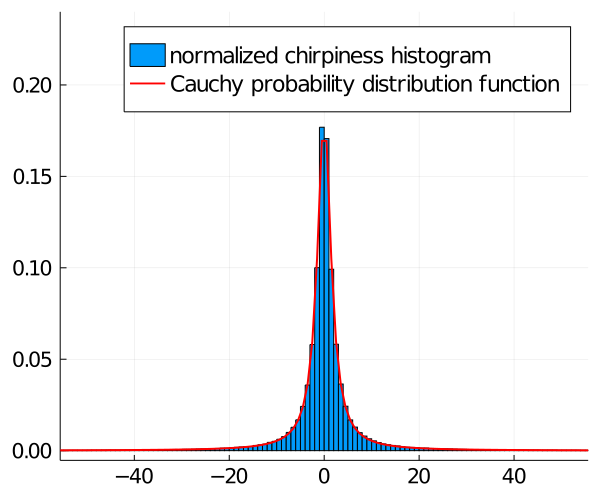
\includegraphics[width=\textwidth]{img/cauchy_dist_pdf.png}
    \caption{Chirpiness of a speech signal compared to Cauchy distribution}
    \label{fig:cauchy_dist}
    \end{minipage}%
    \hfill
    \begin{minipage}{.47\linewidth}
    \centering
        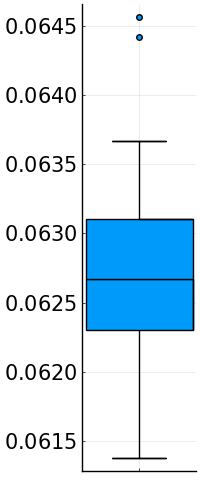
\includegraphics[width=.27\textwidth]{img/cauchy_pt_estimate_iqr_2.png}\hspace{0.1\linewidth}%
        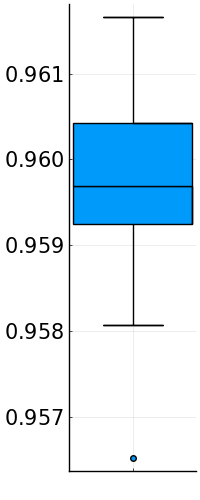
\includegraphics[width=.27\textwidth]{img/cauchy_values_percentage_iqr_2.png}
    \caption{Box plots for estimated Cauchy distributions of speech signals chirpiness.
    \emph{Left:} Kolmogorov-Smirnov statistic values.
    \emph{Right:} percentage of values falling in $I_{0.95}$}
    \end{minipage}
\end{figure}

To overcome this problem, a natural strategy is to model the chirpiness values as
a random variable, and considering only chirpinesses falling inside the confidence
interval \(I_p\) for some reasonable \(p\)-value (e.g., \(p=0.95\)).
A reasonable assumption for the distribution of \(X\) is that it follows
a Cauchy distribution \(\mathrm{Cauchy}(x_0, \gamma)\).
Indeed, this corresponds to assuming that \(\partial_\omega\left\lvert S\right\rvert\) and
\(\partial_\tau\left\lvert S\right\rvert\) are normal (and independent) distributions {[}\protect\hyperlink{ref-papoulis1991}{20}{]}.
As it is customary, we chose as estimator for the location parameter \(x_0\) the median of \(X\)
and for the scale parameter \(\gamma\) half the interquartile distance.

Although statistical tests on a library of real-world speech signals\footnote{The speech material used in the current study is part of an ongoing
  psycholinguistic project on spoken word recognition.
  Speech material comprises 49 Italian words and 118 French words.
  The two sets of words were produced by two (40-year-old) female speakers
  (a French monolingual speaker and an Italian monolingual speaker) and recorded
  using a headset microphone AKG C 410 and a Roland Quad Capture audio interface.
  Recordings took place in the soundproof cabin of the Laboratoire de Phonétique
  et Phonologie (LPP) of Université de Paris Sorbonne-Nouvelle.
  Both informants were told to read the set of words as fluently and naturally as possible}
rejected the assumption that \(X\sim \mathrm{Cauchy}(x_0,\gamma)\),
the fit is quite good according to the Kolmogorov-Smirnov statistic
\(D_n=\sup_x\left\lvert F_n(x)-F_X(x)\right\rvert\). Here, \(F_X\) is the cumulative distribution function
of \(X\) and \(F_n\) is the empirical distribution function
evaluated over the chirpiness values {[}\protect\hyperlink{ref-asswad2021}{2}{]}.

\hypertarget{cortical-activations-in-a1}{%
\subsection{Cortical activations in A1}\label{cortical-activations-in-a1}}

In this model, we consider the primary auditory cortex (A1) as the space of \((\omega,\nu)\in\mathbb{R}^2\).
When hearing a sound signal \(s\), A1 receives its lift to the contact space \(L(t,\omega,\nu)\)
at every instant \(t\).
The \emph{neuron} receives an external charge \(S(t,\omega)\) if \((t,\omega,\nu)\in\Sigma\) and no charge otherwise.

The Wilson-Cowan equations (WC) {[}\protect\hyperlink{ref-wilson1972}{26}{]} have been successfully applied to describe
the evolution of neural activations in V1 as well as A1
{[}\protect\hyperlink{ref-bertalmio2018}{3},\protect\hyperlink{ref-boscain2017}{4},\protect\hyperlink{ref-bressloff2002a}{7},\protect\hyperlink{ref-ermentrout1979}{11},\protect\hyperlink{ref-loebel2007}{17},\protect\hyperlink{ref-rankin2015}{22},\protect\hyperlink{ref-zulfiqar2019}{28}{]}.

The WC equations have the advantage of being flexible as they can be applied independently
of the underlying geometric structure, which is only encoded in the kernel of the integral term.
They allow as well for a natural implementation of delay terms in the interactions
and can be easily tuned via few parameters with clear effect on the results.

In this model, the resulting activation \(a:[0,T]\times\mathbb{R}\times\mathbb{R}\rightarrow\mathbb{C}\) is the solution
to the WC differo-integral equation with a delay \(\delta\).

\begin{equation}
\frac{\partial}{\partial t}a(t,\omega,\nu) = -\alpha a(t,\omega,\nu) + \beta L(t,\omega,\nu)
+ \gamma\int_{\mathbb{R}^2} k_\delta(\omega,\nu\Vert\omega',\nu') \sigma(a(t-\delta,\omega',\nu')) \mathrm{d}\omega'\mathrm{d}\nu'
\end{equation}

where

\begin{itemize}
\tightlist
\item
  \(\alpha,\beta,\gamma>0\) are parameters
\item
  \(\sigma:\mathbb{C}\rightarrow\mathbb{C}\) is a non-linear sigmoid where \(\sigma(\rho e^{i\theta})=\tilde\sigma(\rho)e^{i\theta}\)
  with \(\tilde\sigma(x)=\min\left\{\max\left\{0,\kappa x\right\}, 1\right\},\forall x\in\mathbb{R}\) given a fixed \(\kappa>0\).
\item
  \(k_\delta(\omega,\nu\Vert\omega',\nu')\) is a weight modeling the interaction
  between \((\omega,\nu)\) and \((\omega',\nu')\) after a delay \(\delta>0\) via the kernel of the transport-diffusion
  operator associated to the contact structure of A1.
\end{itemize}

When \(\gamma=0\), the WC equation becomes a standard low-pass filter \(\partial_t a=-\alpha a + L\)
whose solution is simply

\begin{equation}
a(t,\omega,\nu) = \int_0^t e^{-\alpha(s-t)}L(t,\omega,\nu)\mathrm{d}s
\end{equation}

With \(\gamma\neq0\), a non-linear delayed interaction term is added on top
of the low-pass filter, encoding the inhibitory and excitatory interconnections between neurons {[}\protect\hyperlink{ref-boscain2021}{5}{]}.

In the scope of the internship, no work was carried on the integral kernel.
Hence, no further explanation on the WC model is needed.

\pagebreak

\hypertarget{implementation}{%
\section{Implementation}\label{implementation}}

Julia is a relatively new language, it first appeared in 2012,
and its version 1.0 was released in 2018.
The language was built to be fast, general-purpose, dynamic,
and highly technical {[}\protect\hyperlink{ref-julia2018}{1}{]}.

Julia respresents a great alternative for scientific computing
and visualization to replace C/C++, Fortran, Python, Matlab, and R.
It is designed to have the speed of C and Fortran,
with the ease of use of Python, Matlab, and R.
All while maintaining a great syntax for general purpose programming.

Julia is a serious contender as a scientific programming language.
However, the Julia community is still considerabely smaller
than other scientific programming languages.
For instance, in the 2021 Stack Overflow Developer Survey,
1.29\% responded they wanted to work in Julia over the next year
against 48.24\% in Python and 4.66\% in Matlab {[}\protect\hyperlink{ref-so_survey2021}{29}{]}.
As a result, Julia has less stable scientific libraries than
other languages.

\hypertarget{the-wca1.jl-library}{%
\subsection{\texorpdfstring{The \texttt{WCA1.jl} library}{The WCA1.jl library}}\label{the-wca1.jl-library}}

The model was first implemented by Dario Prandi,
allowing to present a series of experiments on simple synthetic sounds.
The code and the experiments are available at
\href{https://github.com/dprn/WCA1}{\texttt{https://github.com/dprn/WCA1}}.

The work I carried on during the internship was built on top of the original code,
my contributions are available at
\href{https://github.com/rand-asswad/WCA1}{\texttt{https://github.com/rand-asswad/WCA1}},
which is forked from the original repository.

Indeed, rewriting the code was necessary in order to experiment
on real sound signals as they are considerabely larger,
otherwise the code would run for a long time and in some cases
errors would arise.
Moreover, an official scientific package should be well-written
and well-documented, and should also try to respect Julia's
code style and recommendations.

\hypertarget{the-stft-module}{%
\subsubsection{The STFT module}\label{the-stft-module}}

Reimplementing the STFT module was necessary in order to carry out
experiments on real sound signals, the preexisting code was not well
adapted for such signals.
Furthermore, an inverse STFT implementation is missing from the Julia
standard libraries such as \href{https://juliapackages.com/p/fftw}{\texttt{FFTW.jl}}
and \href{https://juliapackages.com/p/dsp}{\texttt{DSP.jl}}.
Hence, I researched efficient algorithms for implementing the inverse STFT
and landed on the Griffin-Lim algorithm {[}\protect\hyperlink{ref-griffin1983}{12}{]}.

\begin{figure}
\centering
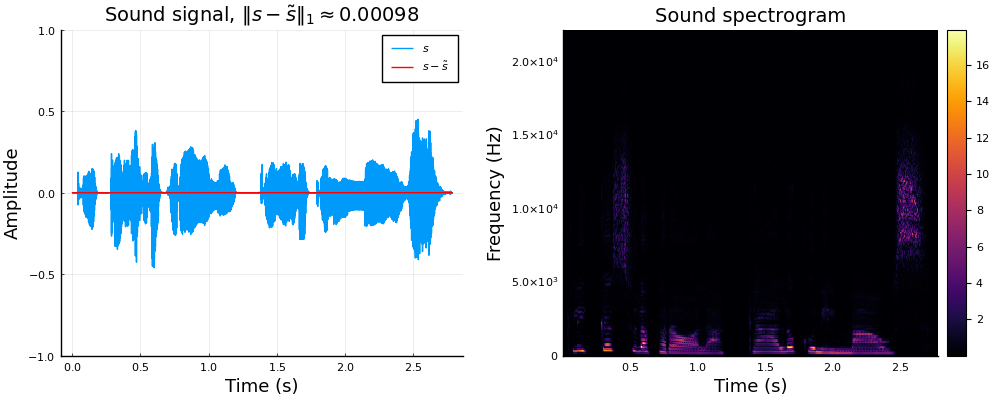
\includegraphics{img/stft_istft.png}
\caption{Left: speech sound \(s\) compared with \(\tilde s=\mathrm{STFT}^{-1}\left\{\mathrm{STFT}\left\{s\right\}\right\}\). Right: spectrogram \(\left\lvert S\right\rvert(\tau,\omega)=\left\lvert\mathrm{STFT}\left\{s(t)\right\}\right\rvert\)}
\end{figure}

\hypertarget{optimizing-the-lift-module}{%
\subsubsection{Optimizing the lift module}\label{optimizing-the-lift-module}}

The sound chirpiness is computed by calculating gradient of the spectrum matrix \(\nabla\left\lvert S\right\rvert\),
which gives the chirpiness with respect to each time-frequency pair

\begin{equation}
\nu(\tau,\omega) =
\begin{cases}
-\frac{\partial_\tau\left\lvert S\right\rvert(\tau,\omega)}{\partial_\omega\left\lvert S\right\rvert(\tau,\omega)} & \text{if}~\left\lvert\partial_\omega\left\lvert S\right\rvert(\tau,\omega)\right\rvert>\varepsilon\\
0 & \text{otherwise}
\end{cases}
\end{equation}

where \(\varepsilon\) is a small threshold.

Afterwards, the chirpiness values are compared to a Cauchy distribution, allowing to establish
a confidence interval \(I_p\) (we take \(p=0.95\)), in order to cut the tails that extend
over the entire real line.

The chirpiness values \(\nu\in I_p=[\nu_{\min},\nu_{\max}]\) are then discretized as the following:
Let \((\nu_n)_{1\leq n\leq N}\) such that \(\nu_{\min}=\nu_1<\cdots<\nu_N=\nu_{\max}\).
Each value \(\nu\) is rounded to the nearest \(\nu_n\).

\begin{equation}
n(\nu) = \left\lfloor\frac{\nu - \nu_{\min}}{\nu_{\max}- \nu_{\min}}(N-1) + 1\right\rceil,\quad\forall\nu\in I_p
\end{equation}
where \(\left\lfloor\cdot\right\rceil:\mathbb{R}\rightarrow\mathbb{Z}\) is the rounding function to the nearest integer.

This was optimized by implementing the function in a variety of ways,
then benchmarking the time and memory consumption for each implementation
over every sample sound from the speech library.
We noticed that the rounding function \(n(\nu)\) can be rewritten
as an affine function with respect to \(\nu\), avoiding to do the same
operations inside the loop, thus saving time and memory.
The explicit expression and the affine expression were both implemented
using a traditional loop, list comprehension, and Julia's broadcast operator.
The list comprehension was clearly the fastest, without compromising
the function's readability nor memory consumption.

\begin{figure}[H]
    \begin{minipage}{.6\linewidth}
    \centering
    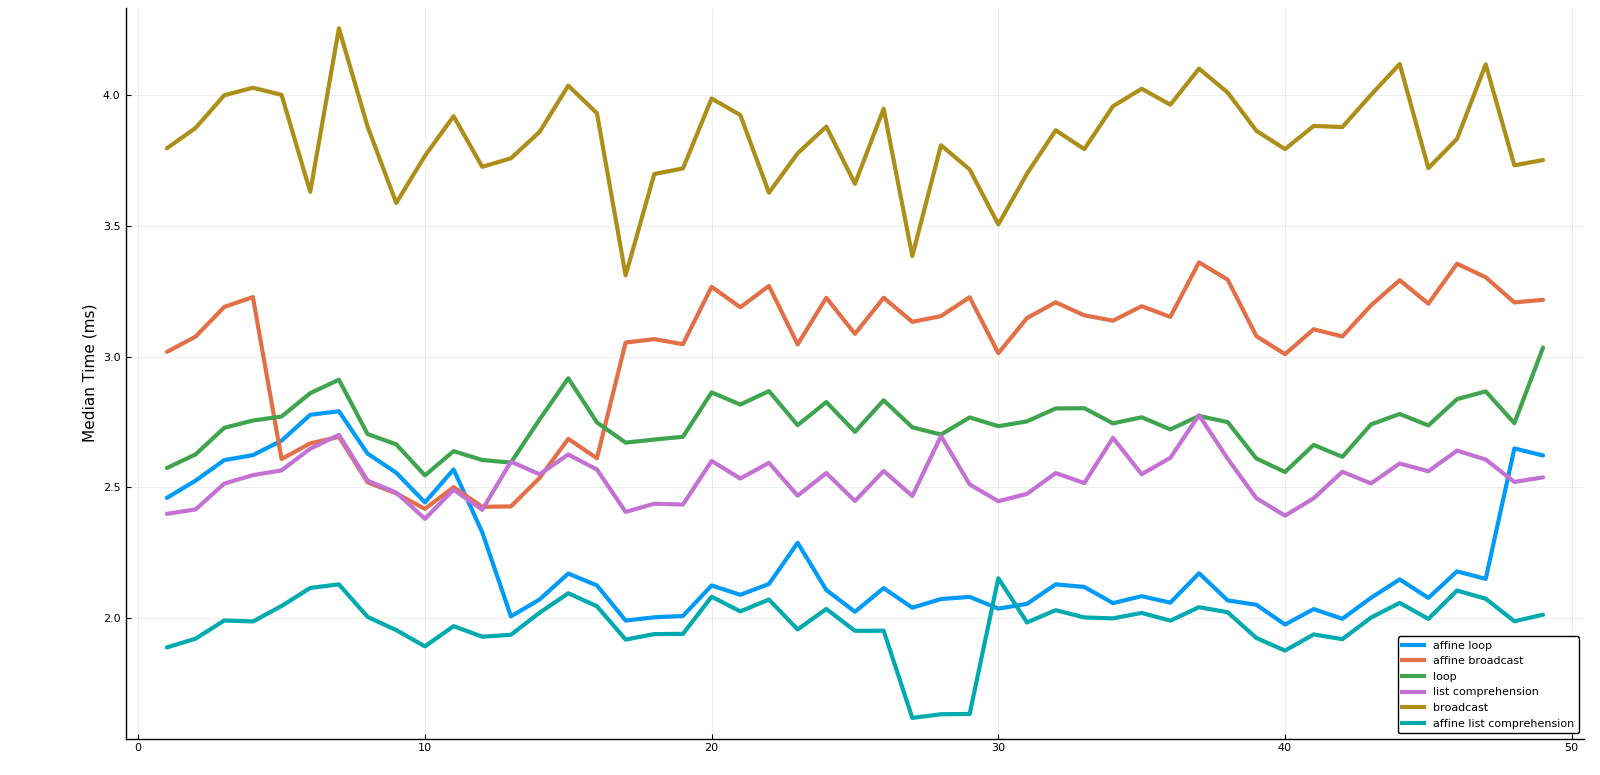
\includegraphics[width=\textwidth]{img/benchmark_median_time.png}
    \caption{The benchmarked median time for each method ploted against the speech samples}
    \label{fig:benchmark_median_time}
    \end{minipage}%
    \hfill
    \begin{minipage}{.35\linewidth}
    \centering
    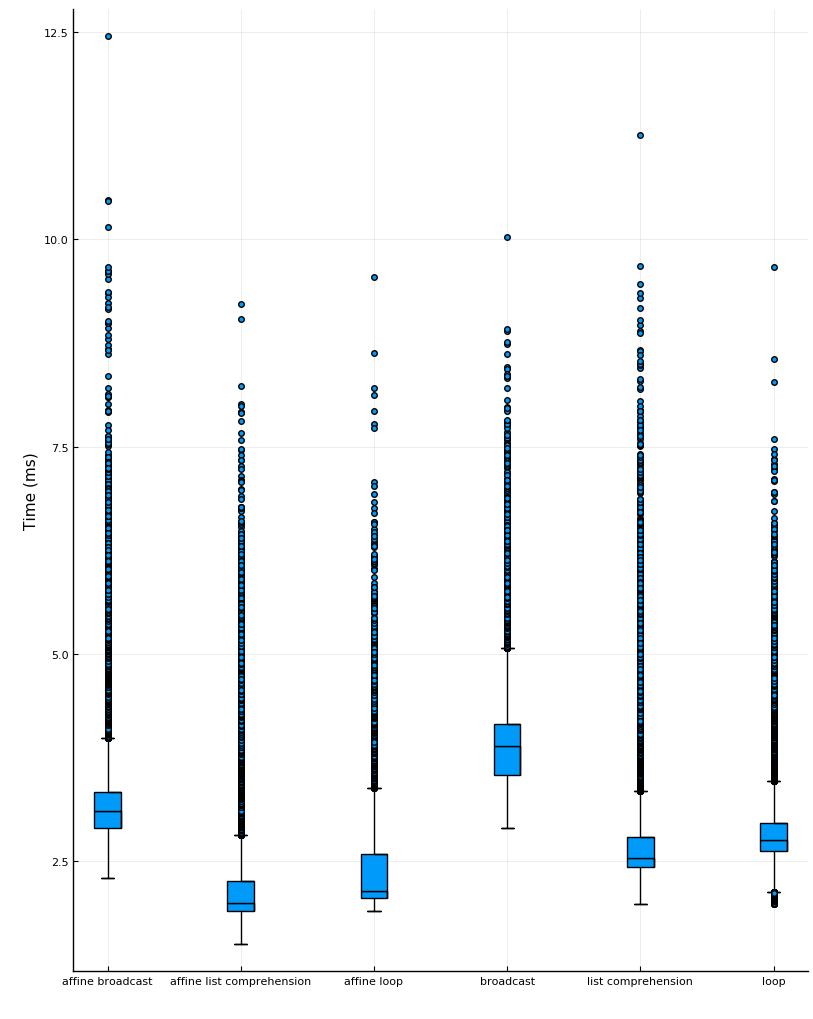
\includegraphics[width=\textwidth]{img/benchmark_time_boxplot.png}
    \caption{Box plots of the benchmarked time for each method on the samples from the speech library}
    \end{minipage}
\end{figure}

It is worth noting that all of the tested methods outperform
the preexisting implementation which had redundant loops
for memory allocation and variable assignment.

\hypertarget{results}{%
\subsection{Results}\label{results}}

\begin{figure}[H]
    \begin{minipage}{.47\linewidth}
    \centering
    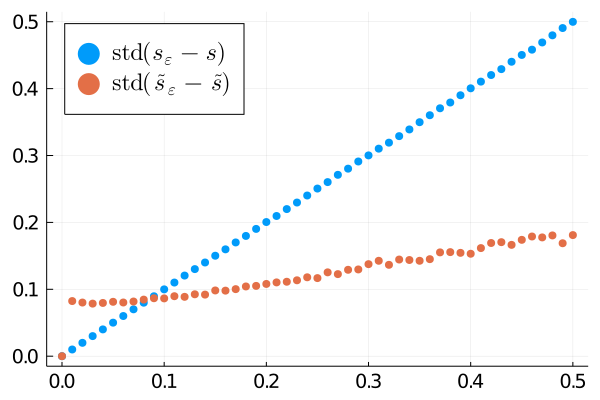
\includegraphics[width=\textwidth]{img/std_diff.png}
    \end{minipage}%
    \hfill
    \begin{minipage}{.47\linewidth}
    \centering
    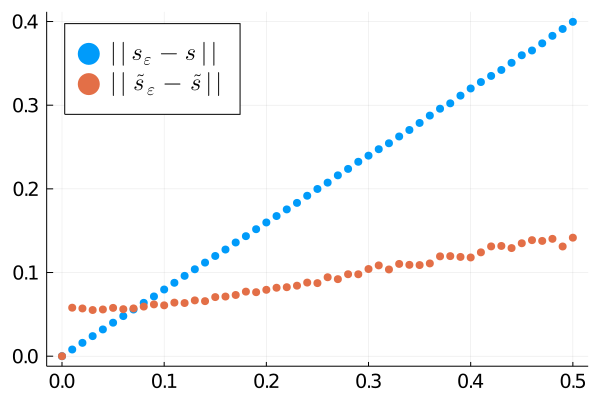
\includegraphics[width=\textwidth]{img/norm_diff.png}
    \end{minipage}
    \caption{\label{fig:experiments}Distance of noisy sound to original one before (blue) and after (red) the processing, plotted against the standard deviation of the noise ($\varepsilon$). \emph{Left:} standard deviation metric. \emph{Right:} $\left\lVert\cdot\right\rVert$ norm.}
\end{figure}

In the figure above, we present the results of the algorithm applied to a denoising task.
Namely, given a sound signal \(s\), we let \(s_\varepsilon= s + g_\varepsilon\),
where \(g_\varepsilon\sim \mathcal N(0,\varepsilon)\) is a gaussian random variable.
We then apply the proposed sound processing algorithm to obtain \(\tilde s_\varepsilon\).
As a reconstruction metric we present both the norm \(\left\lVert\cdot\right\rVert\)
where for a real signal \(s\), \(\left\lVert s\right\rVert = \left\lVert s\right\rVert_1/\dim(s)\)
with \(\left\lVert\cdot\right\rVert_1\) as the \(L_1\) norm
and the standard deviation \(\mathrm{std}(\tilde s_\varepsilon -\tilde s)\).
We observe that according to both metrics the algorithm indeed improves the signal {[}\protect\hyperlink{ref-asswad2021}{2}{]}.

\pagebreak

\hypertarget{conclusion}{%
\section{Conclusion}\label{conclusion}}

So far, we have presented a neuro-geometric model for sound reconstruction,
proposed an implementation of this model in Julia,
and showed results that were published in the GSI 2021 conference proceedings.

In this section we review the model and propose potential
routes for future development.
We explain as well the faced challenges, the acquired knowledge,
and the effect of this internship on my career.

\hypertarget{reviewing-the-model}{%
\subsection{Reviewing the model}\label{reviewing-the-model}}

The proposed model has great potential.
Upon review, many ideas were sought that are worth exploring,
in this section we explain these ideas.
These concepts were to be the basis of a PhD project
under the supervision of Ugo Boscain, Dario Prandi, and Giuseppina Turco.
Unfortunately, we couldn't receive the funding for a PhD
in order to continue working on this fascinating project.

\hypertarget{model-analysis}{%
\subsubsection{Model analysis}\label{model-analysis}}

The promising results obtained on simple synthetic sounds,
suggested possible applications of the model to the problem
of degraded speech {[}\protect\hyperlink{ref-boscain2021}{5}{]}.
The tests on noisy speech were also promising.
However, the tests on cut sound signals were not as impressive.
We were prompted to rethink the lift procedure.

In its current situation, the model lifts the time-frequency representation \(S(\tau,\omega)\)
of a sound to its time-frequency-chirpiness representation \(L(\tau,\omega,\nu)\)
via a heuristic procedure that mimics the naive V1 lift procedure.
This presents three main drawbacks:

\begin{itemize}
\tightlist
\item
  The lifted representation \(L(\tau,\omega,\nu)\), which represents the input fed to an A1 neuron
  \((\omega,\nu)\) at time \(t\), depends strongly on the phase factor of \(S(\tau,\omega)\in\mathbb{C}\).
  This is unrealistic, since (roughly speaking) the cochlea only transmits the spectrogram
  \(\left\lvert S(\tau,\omega)\right\rvert\) as A1 is insensitive to phase.
\item
  At a fixed time \(t>0\), the resulting representation \(L(t,\omega,\nu)\) is a distribution,
  concentrated on a one dimensional curve in the frequency-chirpiness space.
  This is again unrealistic.
\item
  The current procedure to obtain \(L(\tau,\omega,\nu)\) requires to first compute \(S(\tau,\omega)\)
  and then to ``lift'' it.
  This is not satisfactory from a computational point of view, where one would like to have
  a streamlined procedure that yield the input \(L\) directly from the original signal.
\end{itemize}

To improve the model, it is crucial to devise a novel lift procedure allowing to bypass these problems.

\begin{figure}
\centering
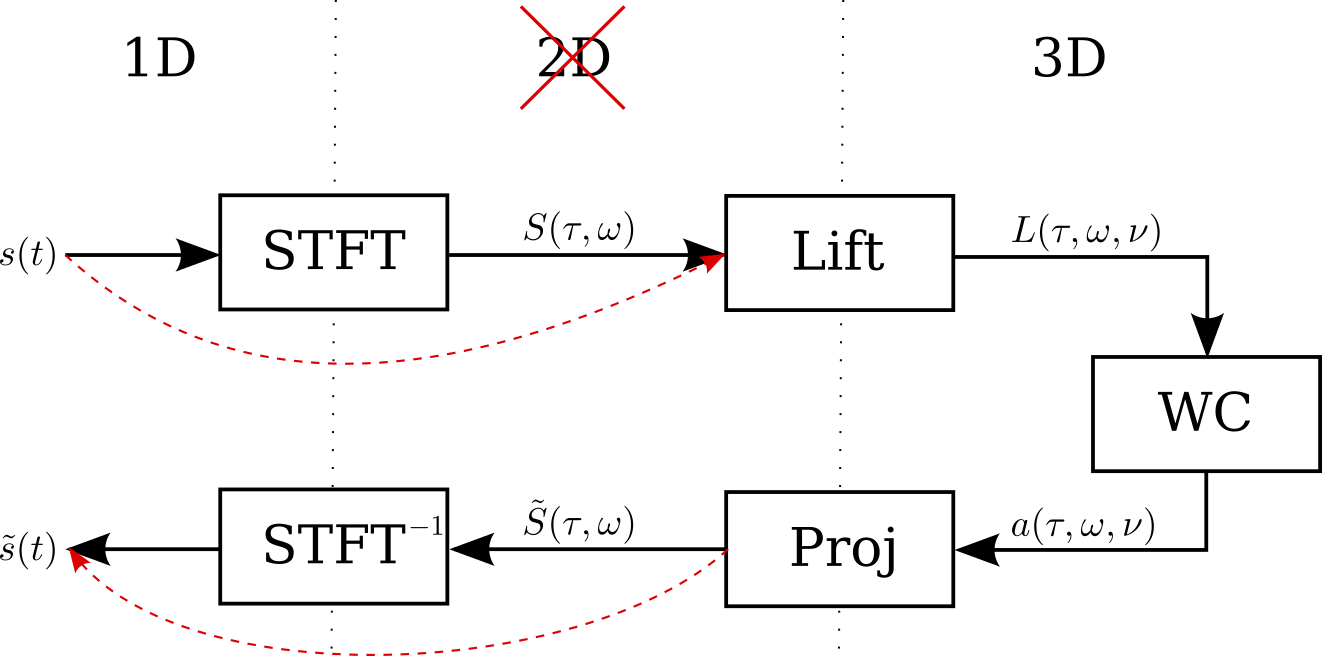
\includegraphics[width=0.7\textwidth,height=\textheight]{img/new_pipeline.png}
\caption{Alternative sound reconstruction pipeline}
\end{figure}

\hypertarget{wavelet-transform}{%
\subsubsection{Wavelet transform}\label{wavelet-transform}}

Taking the V1 models as inspiration, it is interesting to apply wavelet analysis techniques
in order to construct a reasonable structure for the A1 receptive fields,
respecting the symmetries that have already been identified in {[}\protect\hyperlink{ref-boscain2021}{5}{]}.
This work should be deeply connected with important signal processing concepts,
usually applied to the analysis of radar signals {[}\protect\hyperlink{ref-mann1992}{18}{]}.

We started reading state-of-the-art literature on the neurophysiology of the inner ear,
it was clear that a Wavelet transform represents the signal processing
in the cochlea than the STFT transform {[}\protect\hyperlink{ref-reimann2011}{23},\protect\hyperlink{ref-yang1992}{27}{]}.
It is worth mentioning that we studied extensively the auditory representation
of acoustic signals by Yang, Wang, and Shamma {[}\protect\hyperlink{ref-yang1992}{27}{]} in order
to rethink the model of sound processing in the cochlea.

The Wavelet Transform (WT) of a realizable signal \(s\in L^2(\mathbb{R})\) along
a wavelet \(\psi\in L^2(\mathbb{R})\) is defined by

\begin{equation}
W_\psi s(a,t) = \frac{1}{\sqrt{a}} \int_\mathbb{R}s(\tau) \overline{\psi\left(\frac{\tau-t}{a}\right)} \mathrm{d}\tau
\end{equation}
where \(a\) is the dilation variable.

Generally, the WT has a major advantage over the STFT, which is that the time resolution
increases for higher frequencies in the WT.

\begin{figure}
\centering
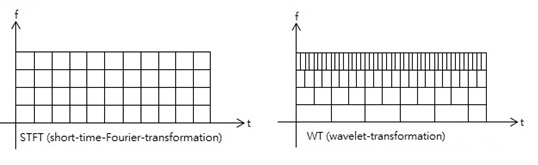
\includegraphics{img/stft_vs_wt.jpg}
\caption{Time resolution in the STFT and the WT {[}\protect\hyperlink{ref-stft_vs_wt}{9}{]}}
\end{figure}

Nevertheless, the WT is given in function of time \(t\) and the dilation variable \(a\).
While \(a\) implicitly represents the frequency, obtaining the chirpiness
is not as straightforward as in the case of the STFT.
In fact, we haven't been able to define an appropriate lift from the WT.
However, the WT represents a path worth exploring more for improving the model.

\hypertarget{the-lift-operator}{%
\subsubsection{The lift operator}\label{the-lift-operator}}

We have seen the definition of the STFT operator \(V_\gamma\) in equation (\ref{eq:stft_operator})
from unitary time and frequency shift operators \(T_\tau,M_\omega\in\mathcal{U}(L^2(\mathbb{R}))\).
A mathematically elegant solution to the lift problem is to introduce
a unitary operator \(C_\nu\) on realizable signals \(s\in L^2(\mathbb{R})\) such that

\begin{equation}
L_\gamma s(\tau,\omega,\nu) = \left\langle s,C_\nu M_\omega T_\tau \gamma\right\rangle_{L^2(\mathbb{R})}
\end{equation}

such an operator would be mathematically stable and computationally cheap.
Unfortunately, no such result was obtained, only further exploration
would reveil if such representation is possible.

\hypertarget{the-group-representation}{%
\subsubsection{The group representation}\label{the-group-representation}}

The quest of redefining the sound lift to the contact space from the Wavelet
transform time-frequency representation started by studying the group representation of the model.

Developing the group representation of the time-frequency representation ended up
confirming both models.
Unfortunately, the work didn't result in a mathematical definition of the chirpiness
(see Appendix \ref{heisenberg}).
Nevertheless, the established work would serve as a basis for further exploration.

\hypertarget{the-wca1.jl-package}{%
\subsubsection{\texorpdfstring{The \texttt{WCA1.jl} package}{The WCA1.jl package}}\label{the-wca1.jl-package}}

The new implementation qualifies as a Julia package,
given the quality of the code with respect to efficiency and its documentation.

Hence, once the model is adjusted, the resulting code should be released
as a free open-source Julia package.
Which would contribute to the quite immature sound signal processing ecosystem
in Julia (alongside \texttt{DSP.jl} and \texttt{WAV.jl}).
Finally, the resulting code should be published on JOSS (the Journal of Open Source Software).

\hypertarget{a-sparse-lift-implementation}{%
\subsubsection{A sparse lift implementation}\label{a-sparse-lift-implementation}}

I noticed that the lifted sound representation \(L[\tau,\omega,\nu]\) was sparse 3D array.
This quality would save a lot of memory since in our samples the ratio of non-zero
elements in \(L\) was under \(10\%\).

Nevertheless, Julia does not have a standard implementation for sparse 3D arrays.
I therefore proceeded to research and implement a hashmap-based (dictionary) sparse 3D array
on top of Julia's standard \texttt{AbstractSparseArray} interface.
My implementation would occupy under \(15\%\) of the memory.
However, the computation speed is considerably less as the hashmap-based approach
for encoding sparse 3D arrays is far from optimal.
An alternative more efficient approach could be considered for implementing such module
without compromising the algorithm's speed.

\hypertarget{acquired-knowledge}{%
\subsection{Acquired knowledge}\label{acquired-knowledge}}

The presented model is clearly complex and interdisciplinary.
The mission requires a deep understanding of fundamental mathematics,
namely geometry, control theory, and group representations,
as well as applied mathematics skills such as
signal processing and numerical analysis.

While the general mission of the internship was known beforehand,
the tasks I had to carry out where changed in light of new results
and my role evolved throughout the internship.

I first needed to familiarize myself with the accomplished work,
a preliminary study of the image reconstruction was needed
in order to understand the sound model and the challenges that are
faced in adapting the initial model for sound reconstruction.
This triggered learning new mathematical concepts.
I did a general reading of \emph{Foundations of Time-Frequency Analysis} by Gröchenig {[}\protect\hyperlink{ref-grochenig2001}{13}{]}
which served as a reference throughout the internship.
While I had a working understanding of basic Fourier analysis thanks to INSA courses
and a familiarity of the Uncertainty Principle and the Short-Time Fourier Transform
thanks to my work on music information retreival for my final Master's project.
The book explains these principles rigourously and also serves as a great source
for learning about the Heisenberg Group and Wavelet Transforms which are the basis
of the proposed model.

Moreover, studying the existing litterature on the subject and working
the mathematical model helped me learn domains
of fundamental and applied mathematics that were new to me.

In addition, co-writing a conference paper and attending the conference
of Geometric Science of Information was an outstanding experience
that I am for extremely grateful.

Finally, the model is implemented in Julia code, which was a new programming language for me,
I therefore learned Julia to be able to improve the existing code.
Having a great basis in low-level and high-level languages,
undoubtedly due to my INSA education and internships,
I was able to write Julia code in very little time.
Nevertheless, it was very important to me to learn
Julia norms and common practices to write elegant and modular code,
as well as learning the mechanisms of this high-level language
in order to optimize the code's performance.
This deeper knowledge of Julia was gained in the following months.

\hypertarget{my-future-project}{%
\subsection{My future project}\label{my-future-project}}

This internship has widened my horizons even more than I had hoped.
I have been more and more interested in pursuing a career in academic research
for the last few years.
Nevertheless, this internship has allowed me to confirm my interest
in such career.
I also gained an appreciation for geometry and analysis.

While I didn't get the opportunity to pursue a PhD thesis in this project,
I have decided, with the help and guidance of my supervisors, to enroll in a
theoretical mathematics Master's degree at University of Lorraine in Nancy.
The program focuses on PDEs and control theory from a theoretical point of view,
which would allow me, combined with my skills in applied mathematics that
I cultivated at INSA Rouen Normandie, to pursue a PhD in these domains.

\pagebreak

\hypertarget{references}{%
\section*{References}\label{references}}
\addcontentsline{toc}{section}{References}

\hypertarget{refs}{}
\leavevmode\hypertarget{ref-julia2018}{}%
{[}1{]} Viral Shah al Stefan Karpinski. Announcing the release of Julia 1.0. Retrieved August 17, 2021 from \url{https://julialang.org/blog/2018/08/one-point-zero/}

\leavevmode\hypertarget{ref-asswad2021}{}%
{[}2{]} Rand Asswad, Ugo Boscain, Giuseppina Turco, Dario Prandi, and Ludovic Sacchelli. 2021. An Auditory Cortex Model for Sound Processing.. 56--64. DOI:\url{https://doi.org/10.1007/978-3-030-80209-7_7}

\leavevmode\hypertarget{ref-bertalmio2018}{}%
{[}3{]} Marcelo Bertalmío, Luca Calatroni, Valentina Franceschi, Benedetta Franceschiello, and Dario Prandi. 2018. A cortical-inspired model for orientation-dependent contrast perception: A link with Wilson-Cowan equations. \emph{arXiv:1812.07425 {[}cs{]}} (December 2018). Retrieved November 12, 2020 from \url{http://arxiv.org/abs/1812.07425}

\leavevmode\hypertarget{ref-boscain2017}{}%
{[}4{]} Ugo Boscain, Roman Chertovskih, Jean-Paul Gauthier, Dario Prandi, and Alexey Remizov. 2017. Cortical-inspired image reconstruction via sub-Riemannian geometry and hypoelliptic diffusion. In \emph{SMAI 2017 - 8e Biennale Française des Mathématiques Appliquées et Industrielles}, La Tremblade, France, 37--53. DOI:\url{https://doi.org/10.1051/proc/201864037}

\leavevmode\hypertarget{ref-boscain2021}{}%
{[}5{]} Ugo Boscain, Dario Prandi, Ludovic Sacchelli, and Giuseppina Turco. 2021. A bio-inspired geometric model for sound reconstruction. \emph{The Journal of Mathematical Neuroscience} 11, 1 (January 2021), 2. DOI:\url{https://doi.org/10.1186/s13408-020-00099-4}

\leavevmode\hypertarget{ref-bressloff2002}{}%
{[}6{]} Paul C. Bressloff and Jack D. Cowan. 2002. An Amplitude Equation Approach to Contextual Effects in Visual Cortex. \emph{Neural Computation} 14, 3 (March 2002), 493--525. DOI:\url{https://doi.org/10.1162/089976602317250870}

\leavevmode\hypertarget{ref-bressloff2002a}{}%
{[}7{]} Paul C. Bressloff, Jack D. Cowan, Martin Golubitsky, Peter J. Thomas, and Matthew C. Wiener. 2002. What Geometric Visual Hallucinations Tell Us about the Visual Cortex. \emph{Neural Computation} 14, 3 (March 2002), 473--491. DOI:\url{https://doi.org/10.1162/089976602317250861}

\leavevmode\hypertarget{ref-citti2006}{}%
{[}8{]} G. Citti and A. Sarti. 2006. A Cortical Based Model of Perceptual Completion in the Roto-Translation Space. \emph{Journal of Mathematical Imaging and Vision} 24, 3 (May 2006), 307--326. DOI:\url{https://doi.org/10.1007/s10851-005-3630-2}

\leavevmode\hypertarget{ref-stft_vs_wt}{}%
{[}9{]} Wikimedia Commons. 2013. Resolution difference between the Short-Time Fourier Transform and the Wavelet Transform. Retrieved September 9, 2021 from \url{https://commons.wikimedia.org/wiki/File:STFT_and_WT.jpg}

\leavevmode\hypertarget{ref-dallos1996}{}%
{[}10{]} P. Dallos. 1996. Overview: Cochlear Neurobiology: Springer Handbook of Auditory Research. \emph{The Cochlea: Springer Handbook of Auditory Research} (1996), 1--43. Retrieved August 13, 2021 from \url{https://www.scholars.northwestern.edu/en/publications/overview-cochlear-neurobiology-springer-handbook-of-auditory-rese}

\leavevmode\hypertarget{ref-ermentrout1979}{}%
{[}11{]} G. B. Ermentrout and J. D. Cowan. 1979. A mathematical theory of visual hallucination patterns. \emph{Biological Cybernetics} 34, 3 (October 1979), 137--150. DOI:\url{https://doi.org/10.1007/BF00336965}

\leavevmode\hypertarget{ref-griffin1983}{}%
{[}12{]} D. Griffin and Jae S. Lim. 1983. Signal estimation from modified short-time Fourier transform. \emph{undefined} (1983). Retrieved September 3, 2021 from \url{https://www.semanticscholar.org/paper/Signal-estimation-from-modified-short-time-Fourier-Griffin-Lim/14bc876fae55faf5669beb01667a4f3bd324a4f1}

\leavevmode\hypertarget{ref-grochenig2001}{}%
{[}13{]} Karlheinz Gröchenig. 2001. \emph{Foundations of Time-Frequency Analysis}. Birkhäuser Basel. DOI:\url{https://doi.org/10.1007/978-1-4612-0003-1}

\leavevmode\hypertarget{ref-heinzel2002}{}%
{[}14{]} Gerhard Heinzel, Albrecht Rüdiger, and Roland Schilling. 2002. Spectrum and spectral density estimation by the Discrete Fourier transform (DFT), including a comprehensive list of window functions and some new at-top windows. (2002). Retrieved September 9, 2021 from \url{https://pure.mpg.de/pubman/faces/ViewItemOverviewPage.jsp?itemId=item_152164}

\leavevmode\hypertarget{ref-hoffman1989}{}%
{[}15{]} William C. Hoffman. 1989. The visual cortex is a contact bundle. \emph{Applied Mathematics and Computation} 32, 2 (August 1989), 137--167. DOI:\url{https://doi.org/10.1016/0096-3003(89)90091-X}

\leavevmode\hypertarget{ref-hubel1959}{}%
{[}16{]} D. H. Hubel and T. N. Wiesel. 1959. Receptive fields of single neurones in the cat's striate cortex. \emph{The Journal of Physiology} 148, 3 (1959), 574--591. DOI:\url{https://doi.org/10.1113/jphysiol.1959.sp006308}

\leavevmode\hypertarget{ref-loebel2007}{}%
{[}17{]} Alex Loebel, Israel Nelken, and Misha Tsodyks. 2007. Processing of sounds by population spikes in a model of primary auditory cortex. \emph{Frontiers in Neuroscience} 1, 1 (November 2007), 197--209. DOI:\url{https://doi.org/10.3389/neuro.01.1.1.015.2007}

\leavevmode\hypertarget{ref-mann1992}{}%
{[}18{]} S. Mann and S. Haykin. 1992. 'Chirplets' and 'warblets': Novel time-frequency methods. \emph{Electronics Letters} 28, (January 1992), 114. DOI:\url{https://doi.org/10.1049/el:19920070}

\leavevmode\hypertarget{ref-muller2015}{}%
{[}19{]} Meinard Müller. 2015. \emph{Fundamentals of Music Processing - Audio, Analysis, Algorithms, Applications}. Springer. Retrieved from \url{https://www.audiolabs-erlangen.de/fau/professor/mueller/bookFMP}

\leavevmode\hypertarget{ref-papoulis1991}{}%
{[}20{]} Athanasios Papoulis. 1991. \emph{Probability, random variables and stochastic processes} (3rd ed.). McGraw-Hill Companies.

\leavevmode\hypertarget{ref-petitot1999}{}%
{[}21{]} Jean Petitot and Yannick Tondut. 1999. Vers une neurogéométrie. Fibrations corticales, structures de contact et contours subjectifs modaux. \emph{Mathématiques et Sciences Humaines} 145, (1999), 5--101. Retrieved August 13, 2021 from \url{https://eudml.org/doc/94522}

\leavevmode\hypertarget{ref-rankin2015}{}%
{[}22{]} James Rankin, Elyse Sussman, and John Rinzel. 2015. Neuromechanistic Model of Auditory Bistability. \emph{PLoS computational biology} 11, 11 (November 2015), e1004555. DOI:\url{https://doi.org/10.1371/journal.pcbi.1004555}

\leavevmode\hypertarget{ref-reimann2011}{}%
{[}23{]} Hans Martin Reimann. 2011. Signal processing in the cochlea: The structure equations. \emph{The Journal of Mathematical Neuroscience} 1, 1 (June 2011), 5. DOI:\url{https://doi.org/10.1186/2190-8567-1-5}

\leavevmode\hypertarget{ref-roads2002}{}%
{[}24{]} Curtis Roads. 2002. Microsound. (March 2002). DOI:\url{https://doi.org/10.7551/mitpress/4601.001.0001}

\leavevmode\hypertarget{ref-sen2014}{}%
{[}25{]} Debashis Sen. 2014. The uncertainty relations in quantum mechanics. \emph{Current science} 107, (July 2014), 203--218. DOI:\url{https://doi.org/10.13140/2.1.5183.0406}

\leavevmode\hypertarget{ref-wilson1972}{}%
{[}26{]} Hugh R. Wilson and Jack D. Cowan. 1972. Excitatory and Inhibitory Interactions in Localized Populations of Model Neurons. \emph{Biophysical Journal} 12, 1 (January 1972), 1--24. DOI:\url{https://doi.org/10.1016/S0006-3495(72)86068-5}

\leavevmode\hypertarget{ref-yang1992}{}%
{[}27{]} Xiaowei Yang, Kuansan Wang, and Shihab Shamma. 1992. Auditory representations of acoustic signals. \emph{Information Theory, IEEE Transactions on} 38, (April 1992), 824--839. DOI:\url{https://doi.org/10.1109/18.119739}

\leavevmode\hypertarget{ref-zulfiqar2019}{}%
{[}28{]} Isma Zulfiqar, Michelle Moerel, and Elia Formisano. 2019. Spectro-Temporal Processing in a Two-Stream Computational Model of Auditory Cortex. \emph{Frontiers in Computational Neuroscience} 13, (2019), 95. DOI:\url{https://doi.org/10.3389/fncom.2019.00095}

\leavevmode\hypertarget{ref-so_survey2021}{}%
{[}29{]} 2021. Stack Overflow Developer Survey 2021. Retrieved from \url{https://insights.stackoverflow.com/survey/2021\#section-most-popular-technologies-programming-scripting-and-markup-languages}

\leavevmode\hypertarget{ref-l2s}{}%
{[}30{]} Laboratory of signals and systems L2S Paris-Saclay University. Retrieved July 29, 2021 from \url{https://l2s.centralesupelec.fr/}

\pagebreak

\hypertarget{appendix-appendix}{%
\appendix}


\hypertarget{istft}{%
\section{Inverse Short-Time Fourier Transform}\label{istft}}

Parseval's formula for the Fourier transform can be transposed
to the STFTs of two signals \(s1\), \(s2\) taken over the windows \(w_1\) and \(w_2\) respectively.

\begin{equation}
\left\langle V_{w_1}s_1,V_{w_2}s_2\right\rangle_{L^2(\mathbb{R}^2)} =
    \left\langle s_1,s_2\right\rangle_{L^2(\mathbb{R})} \overline{\left\langle w_1,w_2\right\rangle}_{L^2(\mathbb{R})}
\end{equation}

\begin{proof}
In order to prove Parseval's formula, we use Fubini's theorem
to interchange the order of integration, we assume that $\overline{w_1}w_2\in L^1(\mathbb{R})$.
We also make use of the fact that
\begin{equation}
\delta(t)=\int_\mathbb{R}e^{-2\pi iwt}\mathrm{d}\omega,\quad\forall t\in\mathbb{R}
\end{equation}
where $\delta$ is the Dirac distribution
\begin{align}
\left\langle V_{w_1}s_1,V_{w_2}s_2\right\rangle_{L^2(\mathbb{R}^2)}
&= \int_{\mathbb{R}^2} \left\langle s_1,M_\omega T_\tau w_1\right\rangle \overline{\left\langle s_2,M_\omega T_\tau w_2\right\rangle} \mathrm{d}\tau\mathrm{d}\omega\\
&= \int_{\mathbb{R}^2} \int_\mathbb{R}s_1(t)\overline{M_\omega T_\tau w_1(t)}\mathrm{d}t
               \int_\mathbb{R}\overline{s_2(t')} M_\omega T_\tau w_2(t') \mathrm{d}t' \mathrm{d}\tau\mathrm{d}\omega\\
&= \int_{\mathbb{R}^4} s_1(t)\overline{T_\tau w_1(t)}
    \overline{s_2(t')} T_\tau w_2(t') e^{-2\pi i\omega(t-t')} \mathrm{d}t\mathrm{d}t'\mathrm{d}\tau\mathrm{d}\omega\\
&= \int_{\mathbb{R}^3} s_1(t)\overline{T_\tau w_1(t)} \overline{s_2(t')} T_\tau w_2(t')
    \overline{\int_\mathbb{R}e^{2\pi i\omega(t-t')}\mathrm{d}\omega} \mathrm{d}t\mathrm{d}t'\mathrm{d}\tau\\
&= \int_{\mathbb{R}^3} s_1(t)\overline{T_\tau w_1(t)} \overline{s_2(t')} T_\tau w_2(t')
    \overline{\delta(t-t')} \mathrm{d}t\mathrm{d}t'\mathrm{d}\tau\\
&= \int_{\mathbb{R}^2} s_1(t)\overline{T_\tau w_1(t)}
    \int_\mathbb{R}\overline{s_2(t')} T_\tau w_2(t') \overline{\delta(t-t')}\mathrm{d}t'\mathrm{d}t\mathrm{d}\tau\\
&= \int_{\mathbb{R}^2} s_1(t)\overline{T_\tau w_1(t)} \overline{s_2(t)} T_\tau w_2(t)\mathrm{d}t\mathrm{d}\tau\\
&= \int_\mathbb{R}s_1(t)\overline{s_2(t)} \int_\mathbb{R}\overline{T_\tau w_1(t)} T_\tau w_2(t)\mathrm{d}\tau\mathrm{d}t\\
&= \int_\mathbb{R}s_1(t)\overline{s_2(t)} \int_\mathbb{R}\overline{w_1(t-\tau)} w_2(t-\tau)\mathrm{d}\tau\mathrm{d}t\\
&= \left\langle s_1,s_2\right\rangle_{L^2(\mathbb{R})} \overline{\left\langle w_1,w_2\right\rangle}_{L^2(\mathbb{R})}
\end{align}
\end{proof}

which implies that \(\left\lVert V_w s\right\rVert_2 = \left\lVert s\right\rVert_2 \left\lVert w\right\rVert_2\), and for \(\left\lVert w\right\rVert_2=1\) we have
\begin{equation}\label{eq:isometry}
\left\lVert V_w s\right\rVert_2 = \left\lVert s\right\rVert_2,\quad s\in L^2(\mathbb{R})
\end{equation}

This means that the STFT operator \(V_w\) is an isometry from \(L^2(\mathbb{R})\)
to \(L^2(\mathbb{R}^2)\) if \(\left\lVert w\right\rVert_2=1\).

\begin{thm}{STFT inversion formula}
Let $w,h\in L^2(\mathbb{R})$ with $\left\langle w,h\right\rangle\neq0$. Then for all $s\in L^2(\mathbb{R})$.
\begin{equation}
s(t) = \frac{1}{\left\langle w,h\right\rangle} \iint_{\mathbb{R}^2}V_w s(\tau,\omega)M_\omega T_\tau h(t) \mathrm{d}\omega\mathrm{d}\tau
\end{equation}
\end{thm}

\begin{proof}
Since $V_w s\in L^2(\mathbb{R}^2)$, let $\tilde s\in L^2(\mathbb{R})$ be defined as
\begin{equation}
\tilde s(t) = \frac{1}{\left\langle w,h\right\rangle} \iint_{\mathbb{R}^2}V_w s(\tau,\omega)M_\omega T_\tau h(t) \mathrm{d}\omega\mathrm{d}\tau
\end{equation}
We therefore have, for all $\varphi\in L^2(\mathbb{R})$, using Parseval's formula
\begin{align}
\left\langle\tilde s, \varphi\right\rangle_{L^2(\mathbb{R})}
&= \frac{1}{\left\langle w,h\right\rangle} \iint_{\mathbb{R}^2} V_w s(\tau,\omega) \left\langle M_\omega T_\tau h, \varphi\right\rangle_{L^2(\mathbb{R})} \mathrm{d}\omega\mathrm{d}\tau\\
&= \frac{1}{\left\langle w,h\right\rangle} \iint_{\mathbb{R}^2} V_w s(\tau,\omega) \overline{\left\langle\varphi,M_\omega T_\tau h\right\rangle}_{L^2(\mathbb{R})} \mathrm{d}\omega\mathrm{d}\tau\\
&= \frac{1}{\left\langle w,h\right\rangle} \iint_{\mathbb{R}^2} V_w s(\tau,\omega) \overline{V_h \varphi(\tau,\omega)} \mathrm{d}\omega\mathrm{d}\tau\\
&= \frac{1}{\left\langle w,h\right\rangle} \left\langle V_w s, V_h \varphi\right\rangle_{L^2(\mathbb{R}^2)}\\
&= \left\langle s, \varphi\right\rangle_{L^2(\mathbb{R})}
\end{align}

Since $\left\langle\tilde s,\varphi\right\rangle_{L^2(\mathbb{R})}=\left\langle s,\varphi\right\rangle_{L^2(\mathbb{R})},\forall\varphi\in L^2(\mathbb{R})$
then in the weak sense $\tilde s = s$.
\end{proof}

It is worth noting that this proof is better expressed with concepts of operator algebra.
Let's consider \(F\) a function on \(E\) such that \(F(x)\in B\) forall \(x\in E\),
where \(B\) is a Banach space, we therefore have
\begin{equation}
f = \int_E F(x)\mathrm{d}x\implies \left\langle f,\varphi\right\rangle = \int_E \left\langle F(x),\varphi\right\rangle \mathrm{d}x
\end{equation}
for all \(\varphi\in B^*\) where \(B^*\) is the dual space to \(B\).
Moreover, if the mapping \(\ell(\varphi)\mapsto\int_E \left\langle F(x),\varphi\right\rangle\mathrm{d}x\)
is a bounded linear operator on \(B^*\), then \(\ell\) defines a unique element \(f\in B^{**}\).
If \(B\) is a reflexive Banach space \(\left(B^{**}=B\right)\), we have a \(f\in B\).
In our case, \(E=\mathbb{R}^2\) and \(F\in L^2(\mathbb{R}^2)\). Let \(f\) be defined as
\begin{equation}
s = \iint_{\mathbb{R}^2} F(\tau,\omega)M_\omega T_\tau \gamma \mathrm{d}\omega\mathrm{d}\tau
\end{equation}
The operator \(\ell\) is then defined as
\begin{equation}
\ell(\varphi) = \iint_{\mathbb{R}^2} F(\tau,\omega)\left\langle M_\omega T_\tau \gamma,\varphi\right\rangle_{L^2(\mathbb{R})} \mathrm{d}\omega\mathrm{d}\tau
          = \iint_{\mathbb{R}^2} F(\tau,\omega) \overline{\left\langle V_\gamma \varphi\right\rangle}_{L^2(\mathbb{R})} \mathrm{d}\omega\mathrm{d}\tau
\end{equation}
We prove \(\ell\) is a bounded operator on \(B^*=L^2(\mathbb{R})\) with the help
of the Cauchy-Schwartz inequality and Parseval's formula.

\begin{equation}
\forall\varphi\in L^2(\mathbb{R}),\left\lvert\ell(\varphi)\right\rvert \leq \left\lVert F\right\rVert_2 \left\lVert V_\gamma \varphi\right\rVert_2
= \left\lVert F\right\rVert_2 \left\lVert\gamma\right\rVert_2 \left\lVert\varphi\right\rVert_2
\end{equation}
Which implies that \(\ell\) defines a unique function \(f\in L^2(\mathbb{R})\) such that
\(\left\langle f,\varphi\right\rangle_{L^2(\mathbb{R})} = \ell(\varphi),\forall\varphi\in L^2(\mathbb{R})\).

\hypertarget{heisenberg}{%
\section{Heisenberg group}\label{heisenberg}}

\hypertarget{heisenberg-group-action-on-the-contact-space}{%
\subsection{Heisenberg group action on the contact space}\label{heisenberg-group-action-on-the-contact-space}}

We consider the unitary shift operators \(T_\tau,M_\omega\in\mathcal{U}(L^2(\mathbb{R}))\).
The commutation relation of these unitary operators is given by
\begin{equation}
T_\tau M_\omega T_\tau^{-1} M_\omega^{-1} = e^{-2\pi i\omega\tau} \mathrm{Id}
\end{equation}

Indeed, \(\forall s\in L^2(\mathbb{R})\)
\begin{align}
T_\tau M_\omega T_\tau^{-1} M_\omega^{-1} s(t)
&= T_\tau M_\omega T_\tau^{-1} e^{-2\pi i\omega t} s(t)\\ 
&= T_\tau M_\omega e^{-2\pi i\omega(t+\tau)} s(t+\tau)\\ 
&= T_\tau e^{-2\pi i\omega\tau} s(t+\tau)\\ 
&= e^{-2\pi i\omega\tau} s(t)
\end{align}

We also consider the representation \(U\) from the Heisenberg group \(\mathbb{H}^1\)
defined \(U:\mathbb{H}^1\rightarrow\mathcal{U}(L^2(\mathbb{R}^2))\) by
\begin{equation}
U(\tau,\omega,\lambda) = e^{-2\pi i\lambda}T_\tau M_\omega
\end{equation}

Therefore, the operator algebra generated by the unitary time and frequency shift
operators coincides with the Heisenberg group \(\mathbb{H}^1\) {[}\protect\hyperlink{ref-boscain2021}{5}{]}.

\hypertarget{introducing-the-chirpiness-to-the-heisenberg-group}{%
\subsection{Introducing the chirpiness to the Heisenberg group}\label{introducing-the-chirpiness-to-the-heisenberg-group}}

An automorphism of a group \(G\) is a group isomorphism from \(G\) onto \(G\).

An isomorphism from \((G_1,*)\) to \((G_2,\cdot)\) is a bijective function
\(f:G_1\rightarrow G_2\) such as \(\forall x,y\in G_1\)

\begin{equation}
f(x*y) = f(x)\cdot f(y)
\end{equation}

It follows that the automorphism of a group \((G,\cdot)\) is a bijective function
\(g:G\rightarrow G\) such as \(\forall x,y\in G\)

\begin{equation}\label{eq:aut_g}
g(x\cdot y) = g(x)\cdot g(y)
\end{equation}

Let's consider the affine group group \(H=\mathbb{R}_+\ltimes\mathbb{R}\) equipped with the square matrix multiplication.

\begin{equation}
H = \left\{\left.\begin{pmatrix}a & t\\0 & 1\end{pmatrix}\right\vert a\in\mathbb{R}_+, t\in\mathbb{R}\right\}
\end{equation}

We denote \((a,t)\equiv \begin{pmatrix}a & t\\0 & 1\end{pmatrix}\in H\)

We hence have \((a,t)(b,s)\equiv\begin{pmatrix}a & t\\0 & 1\end{pmatrix}\begin{pmatrix}b & s\\0 & 1\end{pmatrix}=\begin{pmatrix}ab & as+t\\0 & 1\end{pmatrix}\equiv(ab,as+t)\)

In order to find \(\mathrm{Aut}(H)\) we need to define the group action \((H,\psi)\) that verifies (\ref{eq:aut_g})
\begin{equation}\label{eq:aut_h}
\psi((a,t)(b,s)) = \psi(a,t)\psi(b,s)
\end{equation}
We notice that the right conjugation by \(h\) defined as \(\psi_h(x)=h^{-1}xh\)
is a group action verifying (\ref{eq:aut_h}). For all \(x,y\in H\),
\begin{equation}
\psi_h(xy)=h^{-1}xy h=(h^{-1}xh)(h^{-1}yh)=\psi_h(x)\psi_h(y)
\end{equation}
\(\psi_h\) is therefore an inner automorphism of \(H\).

Let \(h=(b,s)\in H\) therefore \(\psi_h\) is defined \(\forall(a,t)\in H\)
\begin{equation}
\psi_h(a,t)=(b,s)^{-1}(a,t)(b,s)=\left(a, \frac{t}{b}+\frac{(a-1)s}{b}\right)
\end{equation}
Let \(h=(b,0)\in H\), the inner automorphism is defined as \(\psi_h(a,t)=(a,t/b)\).

This corresponds to multiplying the chirpiness by \(b\in\mathbb{R}_+\).
Hence allowing to redefine the augmented space of \((\nu,a,t)\)
as the semidirect product \(G=\mathbb{R}\ltimes H\) with respect to \(\psi\in\mathrm{Aut}(H)\).
Nevertheless, further work is needed in order to construct such space
from the Wavelet time-frequency representation.

\end{document}
